%%%%%%%%%%%%%%%%%%%%%%%%%%%%%%%%%%%%%%%%%
% Masters/Doctoral Thesis 
% LaTeX Template
% Version 2.4 (22/11/16)
%
% This template has been downloaded from:
% http://www.LaTeXTemplates.com
%
% Version 2.x major modifications by:
% Vel (vel@latextemplates.com)
%
% This template is based on a template by:
% Steve Gunn (http://users.ecs.soton.ac.uk/srg/softwaretools/document/templates/)
% Sunil Patel (http://www.sunilpatel.co.uk/thesis-template/)
%
% Template license:
% CC BY-NC-SA 3.0 (http://creativecommons.org/licenses/by-nc-sa/3.0/)
%
%%%%%%%%%%%%%%%%%%%%%%%%%%%%%%%%%%%%%%%%%

%----------------------------------------------------------------------------------------
%	PACKAGES AND OTHER DOCUMENT CONFIGURATIONS
%----------------------------------------------------------------------------------------

\documentclass[
11pt, % The default document font size, options: 10pt, 11pt, 12pt
%oneside, % Two side (alternating margins) for binding by default, uncomment to switch to one side
english, % ngerman for German
singlespacing, % Single line spacing, alternatives: onehalfspacing or doublespacing
%draft, % Uncomment to enable draft mode (no pictures, no links, overfull hboxes indicated)
%nolistspacing, % If the document is onehalfspacing or doublespacing, uncomment this to set spacing in lists to single
%liststotoc, % Uncomment to add the list of figures/tables/etc to the table of contents
%toctotoc, % Uncomment to add the main table of contents to the table of contents
%parskip, % Uncomment to add space between paragraphs
%nohyperref, % Uncomment to not load the hyperref package
headsepline, % Uncomment to get a line under the header
%chapterinoneline, % Uncomment to place the chapter title next to the number on one line
%consistentlayout, % Uncomment to change the layout of the declaration, abstract and acknowledgements pages to match the default layout
]{MastersDoctoralThesis} % The class file specifying the document structure

\usepackage[applemac]{inputenc} % Required for inputting international characters
\usepackage[T1]{fontenc} % Output font encoding for international characters
\usepackage{xhfill}
\usepackage{palatino} % Use the Palatino font by default

\usepackage[hyperref, backend=bibtex,style=alphabetic,natbib=true,backref,backrefstyle=none]{biblatex} % Use the bibtex backend with the authoryear citation style (which resembles APA)

\addbibresource{all_my_bib.bib} % The filename of the bibliography

\usepackage[autostyle=true]{csquotes} % Required to generate language-dependent quotes in the bibliography

%----------------------------------------------------------------------------------------
%	MARGIN SETTINGS
%----------------------------------------------------------------------------------------

\geometry{
	paper=a4paper, % Change to letterpaper for US letter
	inner=2.5cm, % Inner margin
	outer=3.8cm, % Outer margin
	bindingoffset=.5cm, % Binding offset
	top=1.5cm, % Top margin
	bottom=1.5cm, % Bottom margin
	%showframe, % Uncomment to show how the type block is set on the page
}

\linespread{1.3}

%----------------------------------------------------------------------------------------
%	MY NEW ENVIRONMENTS AND PACKAGES
%----------------------------------------------------------------------------------------
\usepackage{enumitem}
\usepackage[export]{adjustbox}
\usepackage{epigraph}


\usepackage{amsmath,amsfonts,amsthm,amssymb}
\usepackage{xcolor,colortbl}
\usepackage{subfigure}
\usepackage{multirow}
\usepackage{booktabs}
\usepackage{csquotes}
\usepackage{listings}


\usepackage{tikz}
\usetikzlibrary{mindmap,backgrounds}
\usetikzlibrary{shapes}
\usetikzlibrary{shapes.symbols}
\usetikzlibrary{decorations.pathreplacing}
\usetikzlibrary{decorations.markings}
\usetikzlibrary{arrows}
\usetikzlibrary{patterns}
\usetikzlibrary{calc}
\usetikzlibrary{positioning}
\usetikzlibrary{matrix}
\usetikzlibrary{automata}
\usetikzlibrary{decorations.pathmorphing}
\usetikzlibrary{shapes.callouts}
\usetikzlibrary{decorations.text}

%\usetikzlibrary{tikzmark}
%\usetikzlibrary{decorations.pathreplacing}
%\usetikzlibrary{fadings}
%\pgfkeys{/tikz/.cd,
%  dec_j/.store in=\dec_j,
%  dec_j=0   %% initial value, set to anything so that even if you don't specify a value later, it compiles
%   }


\theoremstyle{remark}
\newtheorem{remark}{Remark}[chapter]
\newtheorem{lemma}{Lemma}{\bfseries}{\itshape}
\newtheorem{definition}{Definition}
\newtheorem{assumption}{Assumption}{\bfseries}{\itshape}
\newtheorem{property}{Property}{\bfseries}{\itshape}
\newtheorem{example}{Example}{\bfseries}{\itshape}
\newtheorem{notation}{Notation}{\bfseries}{\itshape}
\newtheorem{procedure}{Procedure}{\bfseries}{}

\newcommand*{\todo}[1]{\textbf{\textcolor{red}{#1}}}

\newenvironment{psmallmatrix}
  {\left[\begin{smallmatrix}}
  {\end{smallmatrix}\right]}
%----------------------------------------------------------------------------------------
%	MY NOTATIONS
%----------------------------------------------------------------------------------------
\newcommand*{\vLeak}{x}
\newcommand*{\vLeakVec}{\vec{x}}
\newcommand*{\vaLeak}{X}
\newcommand*{\setLeak}{\vec{\mathcal{X}}}
\newcommand*{\vaLeakVec}{\vec{X}}
\newcommand{\setLeakTrain}{\setLeak_{\text{train}}}
\newcommand{\setLeakTest}{\setLeak_{\text{test}}}
\newcommand{\setLeakValidation}{\setLeak_{\text{validation}}}
\newcommand{\setLeakProfiling}{\setLeak_{\text{profiling}}}
\newcommand{\setTargetTrain}{\setTarget_{\text{train}}}
\newcommand{\setTargetTest}{\setTarget_{\text{test}}}
\newcommand{\setTargetValidation}{\setTarget_{\text{validation}}}
\newcommand{\setTargetProfiling}{\setTarget_{\text{profiling}}}

\newcommand*{\vNNOutput}{\ensuremath {\vec{y}}}

\newcommand*{\setData}{\mathcal{D}}
\newcommand*{\sizeSetData}{\lvert\setData\rvert}
\newcommand*{\setDataTrain}{\mathcal{D}_{\text{train}}}
\newcommand*{\setDataTest}{\mathcal{D}_{\text{test}}}
\newcommand*{\setDataValidation}{\mathcal{D}_{\text{validation}}}
\newcommand*{\setDataProfiling}{\mathcal{D}_{\text{profiling}}}
\newcommand*{\setDataAttack}{\mathcal{D}_{\text{attack}}}
\newcommand*{\setTarget}{\mathcal{Y}}
%\newcommand*{\setDataKDA}{\mathcal{D}_{\text{KDA}}}
%\newcommand{\setLeakKDA}{\setLeak_{\text{KDA}}}
%\newcommand{\setTargetKDA}{\setTarget_{\text{KDA}}}


\newcommand*{\sPOI}{\tau} %signal strength


\newcommand*{\publicParRandVar}{E}
\newcommand*{\publicParVar}{e}
\newcommand*{\keyRandVar}{K}
\newcommand*{\keyVar}{k}
\newcommand*{\keyStar}{k^\star}
\newcommand*{\keyVarSet}{\mathcal{K}}
\newcommand*{\sensVar}{z}
\newcommand*{\sensRandVar}{Z}
\newcommand*{\sensVarValue}[1]{s_{#1}}
\newcommand*{\sensVarGenValue}{s}
\newcommand*{\sensVarOneHot}[1]{\vec{s_{#1}}}
\newcommand*{\sensVarSet}{\mathcal{Z}}
\newcommand*{\numClasses}{\lvert\sensVarSet\rvert}
\newcommand*{\nbClasses}{\lvert\sensVarSet\rvert}
\newcommand*{\sensFunction}{f}
\newcommand{\featureSpace}{\mathcal{F}}
\newcommand*{\distinguisher}{\Delta}


\newcommand*{\yyy}{\vec{y}}
\newcommand*{\YYY}{\vec{Y}}
\newcommand*{\www}{\vec{w}}
%\newcommand*{\WWW}{\textbf{W}}
\newcommand*{\vvv}{\vec{v}}
%\newcommand*{\VVV}{\textbf{V}}

\newcommand*{\nbTraces}{N}
\newcommand*{\nbTrainingTraces}{N_t}
\newcommand*{\nbProfilingTraces}{N_p}
\newcommand*{\nbProfilingTracesPerClass}{N_{p,\sensVarGenValue}}
\newcommand*{\nbAttackTraces}{N_a}
\newcommand*{\nbTracesPerClass}[1][\sensVarGenValue]{N_{#1}}
\newcommand*{\guessingEntropy}{\mathrm{GE}}
\newcommand*{\SR}{\mathrm{SR}}
\newcommand*{\newTraceLength}{C}
\newcommand*{\traceLength}{D}
\newcommand*{\AAlpha}{\vec{\alpha}}
\newcommand*{\BBeta}{\vec{\zeta}}
\newcommand*{\covmat}{\textbf{S}}
\newcommand*{\numPoI}{\sharp\mathrm{PoI}}
\newcommand*{\leakFunction}{\phi}
\newcommand*{\LeakFunction}{\boldsymbol{\phi}}
\newcommand*{\noise}{B}
\newcommand*{\Noise}{\vec{B}}
\newcommand*{\extract}{\epsilon}
\newcommand*{\orderRate}{o}
\newcommand*{\guessingVector}{\vec{g}}

\newcommand*{\entropy}{\mathbb{H}}
\newcommand*{\MLmodel}{F}
\newcommand*{\featureSpaceSize}{S}


\newcommand*{\leakageModel}{L}
\newcommand*{\HD}{\mathrm{HD}}
\newcommand*{\HW}{\mathrm{HW}}

\newcommand*{\prob}{\mathrm{Pr}}
\newcommand*{\pdf}{p}
\newcommand*{\mumumu}{\vec{\mu}}

\newcommand*{\measuresMatrix}{\textbf{M}}
\newcommand*{\projectingMatrix}{\textbf{A}}
\newcommand*{\SW}{\textbf{S}_{\textbf{W}}}
\newcommand*{\SB}{\textbf{S}_{\textbf{B}}}
\newcommand*{\ST}{\textbf{S}_{\textbf{T}}}
\newcommand*{\var}{\mathrm{Var}}
\newcommand*{\cov}{\mathrm{Cov}}
\newcommand*{\esperEst}{\hat{\mathbb{E}}}
\newcommand*{\varEst}{\hat{\mathrm{Var}}}
\newcommand*{\esper}{\mathbb{E}}
\newcommand*{\mmm}{\vec{m}}
\newcommand*{\mmmX}{\overline{\vec{x}}}
\newcommand*{\mmmXclass}[1][\sensVarGenValue]{\vec{\mu}_{#1}}
\newcommand*{\mmmY}{\overline{\vec{y}}}
\newcommand*{\varXclass}[1][\sensVarGenValue]{\vec{\varrho}_{#1}}

\newcommand{\MMM}{\textbf{M}}
\newcommand{\MMMclass}[1][\sensVarGenValue]{\vec{M}_{#1}}
\newcommand{\MMMT}{\vec{M}_{T}}
\newcommand{\NNN}{\textbf{N}}
\newcommand{\III}{\textbf{I}}
\newcommand{\numEigenvectors}{Q}
\newcommand{\kernelMatrix}{\textbf{K}}
\newcommand{\nununu}{\vec{\nu}}
\newcommand{\mmmXPhi}{\overline{\Phi(\vec{x}})}
\newcommand{\mmmXclassPhi}[1][\sensVarGenValue]{\overline{\Phi(\vec{x})}^{#1}}


\newcommand*{\aaa}{\textbf{a}}

\newcommand*{\Sbox}{\mathrm{Sbox}}
\newcommand*{\norm}[1]{\left\lVert#1\right\rVert}
\newcommand*{\softmax}{s}

%----------------------------------------------------------------------------------------
% EDITORIAL DEFINITIONS
%----------------------------------------------------------------------------------------
%\newcommand\given[1][\Big]{\:#1\vert\:}

\makeatletter
\newcommand{\@givenstar}[2]{#1\;\middle|\;#2}
\newcommand{\@givennostar}[3][]{#1#2\;#1|\;#3#1}
\newcommand{\given}{\@ifstar\@givenstar\@givennostar}
\makeatother

\DeclareMathOperator*{\argmin}{argmin}
\DeclareMathOperator*{\argmax}{argmax}

\def\etal{\textit{et al.} }
\newcommand {\ie}{{\em i.e.} }
\def\eg{\textit{e.g.} }
\def\via{\textit{via} }
\def\resp{{\em resp.} }
\def\th{$^\text{th}$}

%----------------------------------------------------------------------------------------
%	THESIS INFORMATION
%----------------------------------------------------------------------------------------

\thesistitle{Feature Extraction for Side-Channel Attacks} % Your thesis title, this is used in the title and abstract, print it elsewhere with \ttitle
\supervisor{Emmanuel \textsc{PROUFF}} % Your supervisor's name, this is used in the title page, print it elsewhere with \supname
\examiner{} % Your examiner's name, this is not currently used anywhere in the template, print it elsewhere with \examname
\degree{Docteur} % Your degree name, this is used in the title page and abstract, print it elsewhere with \degreename
\author{Eleonora \textsc{CAGLI}} % Your name, this is used in the title page and abstract, print it elsewhere with \authorname
\addresses{} % Your address, this is not currently used anywhere in the template, print it elsewhere with \addressname

\subject{Informatique} % Your subject area, this is not currently used anywhere in the template, print it elsewhere with \subjectname
\keywords{} % Keywords for your thesis, this is not currently used anywhere in the template, print it elsewhere with \keywordnames
\university{\href{www.sorbonne-universite.fr}{Sorbonne Universit\'e}} % Your university's name and URL, this is used in the title page and abstract, print it elsewhere with \univname
\department{\href{http://department.university.com}{Department or School Name}} % Your department's name and URL, this is used in the title page and abstract, print it elsewhere with \deptname
\group{\href{http://researchgroup.university.com}{Research Group Name}} % Your research group's name and URL, this is used in the title page, print it elsewhere with \groupname
\faculty{\href{http://faculty.university.com}{Faculty Name}} % Your faculty's name and URL, this is used in the title page and abstract, print it elsewhere with \facname

\AtBeginDocument{
\hypersetup{pdftitle=\ttitle} % Set the PDF's title to your title
\hypersetup{pdfauthor=\authorname} % Set the PDF's author to your name
\hypersetup{pdfkeywords=\keywordnames} % Set the PDF's keywords to your keywords
}

\begin{document}

\frontmatter % Use roman page numbering style (i, ii, iii, iv...) for the pre-content pages

\pagestyle{plain} % Default to the plain heading style until the thesis style is called for the body content

%----------------------------------------------------------------------------------------
%	TITLE PAGE
%----------------------------------------------------------------------------------------

\begin{titlepage}

\includegraphics[height = 20mm]{LOGO_SU.jpg}
\hfill

\includegraphics[height = 20mm]{LOGO_LIP6}
\begin{center}

\vspace*{.02\textheight}
{\scshape\huge Sorbonne Universit\'e\par}\vspace{0.3cm} % University name
\textsc{\Large Ecole Doctorale n$^\circ$ 130 }\\
\textsc{\large Informatique, T\'el\'ecommunications, \'Electronique de Paris}\\[0.3cm]
\end{center}
\vspace*{.02\textheight}
\hfill \textsc{\large Laboratoire d'Informatique de Paris 6 }\\
\vspace*{.02\textheight}
\textsc{\large CEA Grenoble - CESTI} \hfill\\
%\small{Centre d'\'Evaluation de la S\'ecurit\'e des Syst\`emes d'Information} \hfill\\
\begin{center}
\noindent
\xrfill[0.7ex]{1pt}{\textsc{\Large Th\`ese de Doctorat}}\xrfill[0.7ex]{1pt} \\[0.3cm] % Horizontal line
{\scshape\huge \bfseries \ttitle\par}\vspace{0.4cm} % Thesis title
\noindent
\xrfill[0.7ex]{1pt}{\textsc{Sp\'ecialit\'e : Informatique}}\xrfill[0.7ex]{1pt} \\[1.0cm] % Horizontal line




%\vspace*{.04\textheight}
%\textsc{Dirig\'ee par }\href{}{\supname}\\
%\textsc{Encadr\'ee par} C\'ecile \textsc{DUMAS}
% 
%\begin{minipage}[t]{0.4\textwidth}
%\begin{flushleft} \large
%\textsc{Par}
%\href{}{\authorname}\\ % Author name - remove the \href bracket to remove the link
%\textsc{Th\`ese de Doctorat de Informatique???}
%\end{flushleft}
%\end{minipage}
%\begin{minipage}[t]{0.4\textwidth}
%\begin{flushright} \large
%\emph{Dirig\'ee par}
%\href{}{\supname}\\% Supervisor name - remove the \href bracket to remove the link  
%\emph{Encadr\'ee par} C\'ecile \textsc{DUMAS}
%\end{flushright}
%\end{minipage}\\[3cm]

\vspace*{.04\textheight}
\large{Pr\'esent\'ee et soutenue publiquement par \textsc{Eleonora CAGLI}}\\
\large{le 05 d\'ecembre 2018}

\end{center}

\vspace*{.04\textheight}

\begin{minipage}[t]{\textwidth}
\vspace*{0.3cm}
\large{Devant un jury compos\'e de :}\\

\textsc{Emmanuel PROUFF, } \textit{ANSSI} \hfill Directeur de th\`ese \\
  \textsc{Louis GOUBIN, } \normalsize{\textit{Universit\'e de 
Versailles$-$St$-$Quentin$-$en$-$Yvelines}} \hfill \large{Rapporteur\\
\textsc{Fran\c{c}ois-Xavier STANDAERT, } \textit{UCL, Belgique} \hfill Rapporteur\\
  \textsc{Olivier RIOUL, } \textit{T\'el\'ecom ParisTech} \hfill Examinateur \\
 \textsc{Annelie HEUSER, } \textit{CNRS} \hfill Examinateur\\
\textsc{Marios CHOUDARY, } \textit{University Politehnica of Bucharest} \hfill Examinateur\\
 \textsc{Yannick TEGLIA, } \textit{Gemalto} \hfill Examinateur\\
 \textsc{C\'ecile DUMAS, } \textit{CEA Grenoble} \hfill Encadrante et membre invit\'e }

\end{minipage}
%\large \textit{A thesis submitted in fulfillment of the requirements\\ for the degree of \degreename}\\[0.3cm] % University requirement text
%\textit{in the}\\[0.4cm]
%\groupname\\\deptname\\[2cm] % Research group name and department name
% 
%\vfill
%
%{\large \today}\\[4cm] % Date
%%\includegraphics{Logo} % University/department logo - uncomment to place it
% 
%\vfill

\end{titlepage}

%----------------------------------------------------------------------------------------
%	DECLARATION PAGE
%----------------------------------------------------------------------------------------

%\begin{declaration}
%\addchaptertocentry{\authorshipname} % Add the declaration to the table of contents
%\noindent I, \authorname, declare that this thesis titled, \enquote{\ttitle} and the work presented in it are my own. I confirm that:
%
%\begin{itemize} 
%\item This work was done wholly or mainly while in candidature for a research degree at this University.
%\item Where any part of this thesis has previously been submitted for a degree or any other qualification at this University or any other institution, this has been clearly stated.
%\item Where I have consulted the published work of others, this is always clearly attributed.
%\item Where I have quoted from the work of others, the source is always given. With the exception of such quotations, this thesis is entirely my own work.
%\item I have acknowledged all main sources of help.
%\item Where the thesis is based on work done by myself jointly with others, I have made clear exactly what was done by others and what I have contributed myself.\\
%\end{itemize}
% 
%\noindent Signed:\\
%\rule[0.5em]{25em}{0.5pt} % This prints a line for the signature
% 
%\noindent Date:\\
%\rule[0.5em]{25em}{0.5pt} % This prints a line to write the date
%\end{declaration}
%
%\cleardoublepage

%----------------------------------------------------------------------------------------
%	QUOTATION PAGE
%----------------------------------------------------------------------------------------

%\vspace*{0.2\textheight}
%
%\noindent\enquote{\itshape Thanks to my solid academic training, today I can write hundreds of words on virtually any topic without possessing a shred of information, which is how I got a good job in journalism.}\bigbreak
%
%\hfill Dave Barry

%----------------------------------------------------------------------------------------
%	ABSTRACT PAGE
%----------------------------------------------------------------------------------------

%\begin{abstract}
%\addchaptertocentry{\abstractname} % Add the abstract to the table of contents
%The Thesis Abstract is written here (and usually kept to just this page). The page is kept centered vertically so can expand into the blank space above the title too\ldots
%\end{abstract}

%----------------------------------------------------------------------------------------
%	ACKNOWLEDGEMENTS
%----------------------------------------------------------------------------------------

\begin{acknowledgements}
\addchaptertocentry{\acknowledgementname} % Add the acknowledgements to the table of contents
%C'est avec grand plaisir que j'utilise cette page de mon manuscrit pour remercier toutes les personnes qui ont eu un rôle dans ce long parcours qui se termine. Je veux remercier qui a permis à ce parcours de commencer et de se terminer, qui m'a donné confiance, qui m'a guidé, qui m'a stimulé, qui m'a encouragé, qui m'a fait douter, et pourquoi pas, qui m'a entravé. \\

Emmanuel a sans doute recouvert une grande partie de ces rôles (mais pas tous !). Sa passion pour la recherche est contagieuse et a été un véritable carburant pendant ces années. Je le remercie pour m'avoir guidé, pour tous les échanges enrichissants que nous avons eu, pour ces enseignements, les idées précieuse qu'il a voulu partager avec moi, et ses encouragements qui n'ont jamais manqué. \\

Je tiens à remercier de cœur Cécile, qui m'a accueilli et suivie au quotidien au sein du CESTI. Je la remercie pour sa disponibilité illimitée, sa confiance ses idées brillantes, et son esprit positif. \\

Je souhaite remercier sincèrement François-Xavier Standaert et Louis Goubin, qui ont été rapporteurs de mon manuscrit, ainsi que Olivier Rioul, qui avait en principe aussi accepté de l'être. Je remercie en outre Philippe Elbaz-Vincent, Annelie Heuser, Yannick Teglia et Marios Choudary pour avoir accepté de prendre part à mon jury de thèse. \\

Je remercie encore François-Xavier Standaert pour m'avoir accueilli une semaine à l'Université Catholique de Louvain-la-Neuve. Même si notre collaboration n'a pas abouti au résultat envisagé par causes diverses et de force majeure, j'ai pu profiter d'échanges très enrichissants avec lui, ainsi que avec Vincent Grosso, Liran Lerman et Anthony Journault, que je remercie également. Je ne veux pas cacher que le séjour à Louvain-la-Neuve, plongée dans un contexte purement académique, a été source de forte motivation pour la poursuite de mes études. \\

Pendant ma thèse, j'ai eu diverses occasions de faire des rencontres aussi beaux que dignes de grands remerciements. Je voudrais remercier toutes les personnes que j'ai rencontré à l'ANSSI, à Louvain-la-Neuve, en conférence ou en école d'été et en particulier à Ilaria, Elizabeth, Siemen, Guillaume, Nicolas, Marjia, Adrien, Dahmun, Aurore, Romain, Colin, Joël et Sonia.

Prima del dottorato, ho incontrato alcune persone che sono state di fondamentale importanza per la mia scelta di intraprendere questo percorso, e che ringrazio di cuore: in primo luogo Lilli e Guido, i cui nomi mi piace scrivere l'uno accanto all'altro nonostante i loro ruoli diametralmente opposti nella mia crescita, ma anche Danilo e Marco.

Ensuite, j'aimerais remercier les personnes que j'ai côtoyé au quotidien pendant ces années, mes (anciens ou présents) collègues du CESTI. Merci en particulier à Louis, mon co-bureau des premières années, pour avoir été pour moi le modèle (injoignable !) de doctorant parfait.  

......................

Pour finir un merci immense aux plus grands obstacles vivants de ma thèse : Giacomo, qui m'a permis d'intégrer à mon projet de thèse quatre déménagements et deux enfants, et mes deux petits Camillo et Ottavio. Merci à vous trois pour votre capacité de m'épuiser et me recharger en même temps, vous êtes la source de toutes mes énergies et mon soutien solide !
\end{acknowledgements}

%----------------------------------------------------------------------------------------
%	LIST OF CONTENTS/FIGURES/TABLES PAGES
%----------------------------------------------------------------------------------------

\tableofcontents % Prints the main table of contents

\listoffigures % Prints the list of figures

\listoftables % Prints the list of tables

%----------------------------------------------------------------------------------------
%	ABBREVIATIONS
%----------------------------------------------------------------------------------------

\begin{abbreviations}{ll} % Include a list of abbreviations (a table of two columns)
\textbf{AES} & \textbf{A}dvanced \textbf{E}ncryption \textbf{S}tandard\\
\textbf{ANSSI} & \textbf{A}gence \textbf{N}ational de la \textbf{S}\'ecurit\'e des \textbf{S}yst\`emes d' \textbf{I}nformation \\
\textbf{CC} & \textbf{C}ommon \textbf{C}riteria\\

\textbf{CESTI} & \textbf{C}entre d'\textbf{E}valuation de la \textbf{S}\'ecurit\'e des \textbf{T}\'echnologies de l'\textbf{I}nformation\\
\textbf{CNN} & \textbf{Convolutional} \textbf{N}eural \textbf{N}etwork\\
\textbf{CPA} & \textbf{C}orrelation \textbf{P}ower \textbf{A}nalysis \\

\textbf{DA} & \textbf{D}ata \textbf{A}ugmentation\\
\textbf{DL} & \textbf{D}eep \textbf{L}earning\\
\textbf{DoM} & \textbf{D}ifference \textbf{o}f \textbf{M}eans \\

\textbf{DPA} & \textbf{D}ifferential \textbf{P}ower \textbf{A}nalysis \\

\textbf{EAL} & \textbf{E}valuation \textbf{A}ssurance \textbf{L}evels \\
\textbf{EGV} & \textbf{E}xplained \textbf{G}lobal \textbf{Variance}\\
\textbf{ELV} & \textbf{E}xplained \textbf{L}ocal \textbf{Variance}\\


\textbf{ETR} & \textbf{E}valuation \textbf{T}echnical \textbf{R}apport\\
\textbf{GE} & \textbf{G}uessing \textbf{E}ntropy\\
\textbf{GPU} & \textbf{G}raphic \textbf{P}rocessing \textbf{U}nit\\
\textbf{HMM} & \textbf{H}idden \textbf{M}arcov \textbf{M}odel \\

\textbf{HOSCA} & \textbf{H}irer-\textbf{O}rder \textbf{S}ide-\textbf{C}hannel \textbf{A}ttack\\

\textbf{IPR} & \textbf{I}nverse \textbf{P}articipation \textbf{R}atio\\

\textbf{ITSEF} & \textbf{I}nformation \textbf{T}echnology \textbf{S}ecurity \textbf{E}valuation \textbf{F}acility \\
\textbf{KDA} & \textbf{K}ernel Fisher \textbf{D}iscriminant \textbf{A}nalysis\\

\textbf{LDA} & \textbf{L}inear \textbf{D}iscriminant \textbf{A}nalysis\\
\textbf{LDC} & \textbf{L}inear \textbf{D}iscriminant \textbf{C}omponent\\

\textbf{MIA} & \textbf{M}utual \textbf{I}formation \textbf{A}nalysis\\
\textbf{MMPC} & \textbf{M}oment against \textbf{M}oment \textbf{P}rofiling \textbf{C}orrelation \\

\textbf{ML} & \textbf{M}achine \textbf{L}earning \ /  \ \textbf{M}aximum-\textbf{L}ikelihood \\
\textbf{MLP} & \textbf{M}ulti-\textbf{L}ayer \textbf{P}erceptron \\

\textbf{MSE} & \textbf{M}ean \textbf{S}quared \textbf{E}rror\\

\textbf{NIST} & \textbf{N}ational \textbf{I}nstitute of \textbf{S}tandards and \textbf{T}echnology \\
\textbf{NN} & \textbf{N}eural \textbf{N}etwork\\

\textbf{PC} & \textbf{P}rincipal \textbf{C}omponent\\

\textbf{PCA} & \textbf{P}rincipal \textbf{C}omponents \textbf{A}nalysis\\
\textbf{PoI} & \textbf{P}oint \textbf{o}f \textbf{I}nterest\\
\textbf{PP} & \textbf{P}rojection \textbf{P}ursuits\\

\textbf{PV} & \textbf{P}rincipal \textbf{V}ariable\\
\textbf{RDI} &\textbf{R}andom \textbf{D}elay \textbf{I}nterrupt \\

\textbf{SAR} &\textbf{S}ecurity \textbf{A}ssurance \textbf{R}equirements \\

\textbf{SCA} & \textbf{S}ide-\textbf{C}hannel \textbf{A}ttack\\
\textbf{SFR} & \textbf{S}ecurity \textbf{F}unctional \textbf{R}equirements \\
\textbf{SNR} & \textbf{S}ignal-to-\textbf{N}oise-\textbf{R}atio \\

\textbf{SoD} & \textbf{S}um \textbf{o}f \textbf{D}ifferences\\
\textbf{SoSD} & \textbf{S}um \textbf{o}f \textbf{S}quared \textbf{D}ifferences\\
\textbf{SoST} & \textbf{S}um \textbf{o}f \textbf{S}quared \textbf{T}-statistics\\

\textbf{SPA} & \textbf{S}imple \textbf{P}ower \textbf{A}nalysis \\
\textbf{SR} & \textbf{S}uccess \textbf{R}ate\\

\textbf{SSS} & \textbf{S}mall \textbf{S}ample \textbf{S}ize problem\\
\textbf{SVM} & \textbf{S}upport \textbf{V}ector \textbf{M}achine \\

\textbf{TA} & \textbf{T}emplate \textbf{A}ttack \\
\textbf{TDNN} & \textbf{T}ime-\textbf{D}elayed \textbf{N}eural \textbf{N}etwork \\

\textbf{TOE} & \textbf{T}arget \textbf{O}f \textbf{E}valuation \\

\end{abbreviations}

%----------------------------------------------------------------------------------------
%	PHYSICAL CONSTANTS/OTHER DEFINITIONS
%----------------------------------------------------------------------------------------

%\begin{constants}{lr@{${}={}$}l} % The list of physical constants is a three column table
%
%% The \SI{}{} command is provided by the siunitx package, see its documentation for instructions on how to use it
%
%Speed of Light & $c_{0}$ & \SI{2.99792458e8}{\meter\per\second} (exact)\\
%%Constant Name & $Symbol$ & $Constant Value$ with units\\
%
%\end{constants}

%----------------------------------------------------------------------------------------
%	SYMBOLS
%----------------------------------------------------------------------------------------

%\begin{symbols}{lll} % Include a list of Symbols (a three column table)
%
%$GF(2^b)$ & Galois Field of order $2^b$\\
%$\mathbb{Z}_N^{*}$ & ...\\
%%$a$ & distance & \si{\meter} \\
%%$P$ & power & \si{\watt} (\si{\joule\per\second}) \\
%%%Symbol & Name & Unit \\
%%
%%\addlinespace % Gap to separate the Roman symbols from the Greek
%%
%%$\omega$ & angular frequency & \si{\radian} \\
%
%\end{symbols}

%----------------------------------------------------------------------------------------
%	DEDICATION
%----------------------------------------------------------------------------------------

\dedicatory{Dedicated to little Ottavio, with me during the redaction of this thesis, from the first to the last word.} 

%----------------------------------------------------------------------------------------
%	THESIS CONTENT - CHAPTERS
%----------------------------------------------------------------------------------------

\mainmatter % Begin numeric (1,2,3...) page numbering

\pagestyle{thesis} % Return the page headers back to the "thesis" style

% Include the chapters of the thesis as separate files from the Chapters folder
% Uncomment the lines as you write the chapters
\part{Context and State of the Art}
% Chapter Template

\chapter{Introduction} % Main chapter title

\label{ChapterIntroduction}

%----------------------------------------------------------------------------------------
%	SECTION 1
%----------------------------------------------------------------------------------------

\section{Introduction to Cryptography}
The terms \emph{Cryptography} (from the Greek \emph{krypt\`os} (secret) and \emph{graphein} (writing)) and \emph{Cryptanalysis}, denotes two branches of a science named \emph{Cryptology}, or \emph{science of the secret}. Cryptography initially refers to the art of \emph{encrypting} messages, which means writing meaningful messages in such a way to appear nonsense to anyone unaware of the encryption process. In general, cryptography aims to construct protocols to secure communication, while cryptanalysis studies the resistance of cryptographic techniques, developing \emph{attacks} to break the cryptosystems' security claims. These two complementary domains evolve in parallels, since the evolution of attack techniques allows conceiving more resistant cryptographic algorithms, and inversely the resistance of such algorithms requires the conception of more sophisticated attacks.\\

The art of cryptography is very ancient, probably as ancient as the language, but only the development of information technology made cryptology take the shape of a proper science, sometimes referred to as \emph{Modern cryptology}. The last be seen as a branch of different disciplines, such as applied mathematics, computer science, electrical engineering, and communication science. Modern cryptosystems exploit algorithms based on mathematical tools and are implemented as computer programs, or electronic circuits. Their goal is to provide security functionality for communications that use \emph{insecure channels}, for example the internet. In particular, modern cryptosystems are designed in order to ensure at least one of the four following information security properties:
\begin{itemize}
\item[a.] \emph{confidentiality}: the transmitted message must be readable only by a chosen pool of authorized entities;
\item[b.] \emph{authenticity}: the receiver can verify the identity of the sender of a message;
\item[c.] \emph{non-repudiation}: the sender of a message cannot deny having sent the message afterwards;
\item[d.] \emph{data integrity}: the receiver can be convinced that the message has not been corrupted during the transmission.


\end{itemize} 

Two branches of cryptography may be distinguished: the \emph{symmetric cryptography} and the \emph{asymmetric cryptography}. The first one historically appeared before and is based on the hypothesis that the two communicating entities share a common secret, or private key; for this reason this is also called \emph{secret key cryptography}. The second one, introduced around 1970, allows any entity to encrypt a message in such a way that only a unique chosen other entity could decrypt it; this is also called \emph{public key cryptography}. \\

A general principle in cryptography, nowadays widely accepted by cryptography researchers, is the one given by Kerckhoff in in 19th century: it states that cryptosystems should be secure even if everything about the system, except the key, is public knowledge. Following this principle, today many industrials and governmental agencies exploit for their security services cryptosystems based over standardized algorithms. Such algorithms are of public domain, thus have been tested and tried to be broken by a large amount of people, before, during and after the standardization process. Resistance to many attempts of attacks is actually the strengths of standard algorithms.\\

In the following part of this section a description of the two standard cryptographic primitives, \emph{i.e.} building block algorithms used to build cryptographic protocols, that will be used in this thesis will; a symmetric one, the AES, and an asymmetric one, the RSA. 
\subsection{Description of AES}
The \emph{Advanced Encryption Standard} (AES) has been standardized in 2001 by the United States governmental agency \emph{National Institute of Standards and Technology} (NIST) through the \emph{Federal Information
Processing Standards Publication 197 } (FIPS PUB 197) \cite{nist197}. It is a symmetric \emph{block cipher}, \emph{i.e.} an algorithm operating on fixed-length groups of bits.\footnote{in contrast with \emph{stream ciphers}, which operate over a single plaintext bit at time} The AES operates on blocks of 128 bits of plaintext, and can use keys of size 128, 192 or 256 bits. The encryption is done by rounds. The number of executed rounds depends on the key size (10 rounds for 128 bits, 12 for 192 and 14 pour 256). The basic unit for processing in the AES algorithm is a byte. For AES internal operations, bytes are arranged on a two-dimensional array of bytes called the \emph{state}, denoted $s$. Such a state has 4 rows and 4 columns, thus contains 16 bytes. The byte lying at the $i$-th row, $j$-th column of $s$ will be denoted by $s_{i,j}$ for $i,j\in\{0,1,2,3\}$. The 16 input bytes and the 16 output bytes are indexed column-wise as shown in Fig.~\ref{fig:AES_state}. Each element $s_{i,j}$ of a state is mathematically seen as an element of the \emph{Rjindael finite field}, defined as $GF(2^8) = \mathbb{Z}/{2\mathbb{Z}[X]}/P(X)$ where $P(X) = X^8 + X^4 + X^3 + X + 1$. Five functions are performed during the AES, named KeySchedule, AddRoundKey, SubBytes, ShiftRow and MixColumn. At high level the AES algorithm is described hereafter:
\begin{itemize}
\item[\textbf{Key Expansion:}]  derivation of round keys from secret key through the KeySchedule function
\item[\textbf{Round 0:} ] 
\begin{itemize}
\item[] AddRoundKey
\end{itemize}
\item[\textbf{Rounds 1 to penultimate:}] 
\begin{itemize}
\item[] SubBytes
\item[] ShiftRow
\item[] MixColumn
\item[] AddRoundKey
\end{itemize}
\item[\textbf{Last Round:}] 
\begin{itemize}
\item[] SubBytes
\item[] ShiftRow
\item[] AddRoundKey
\end{itemize}
\end{itemize}

\begin{figure}
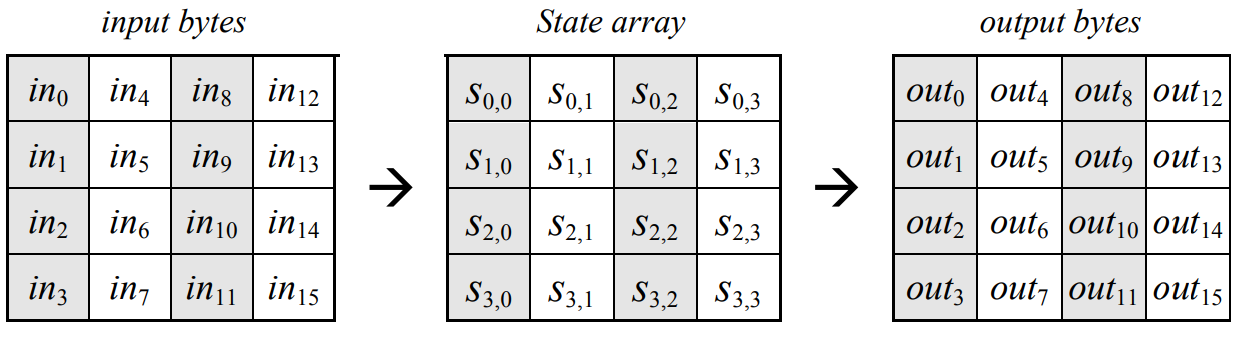
\includegraphics[width = \textwidth]{../Figures/FISP_AES/state.png} 
\caption[State array input and output.]{State array input and output. Source: \cite{nist197}.}\label{fig:AES_state}
\end{figure}

A description of the five functions is provided hereafter.

\subsubsection*{KeySchedule}
The key round of the initial round of AES coincides with the secret encryption key $\boldsymbol{K} = (k_{0,0},k_{0,1},\dots,k_{0,3}, k_{1,0},\dots,k_{1,3},\dots,k_{3,3})$. The $i$-th round key is given by 
\begin{equation*}
\boldsymbol{K_i} = (k_{4i,0},k_{4i,1},\dots,k_{4i,3}, k_{4i+1,0},\dots,k_{4i+1,3},\dots,k_{4i+3,3}),
\end{equation*}
where, for $i>3$
\begin{equation*}
\begin{cases}
k_{a,b} = k_{a-4,b}\oplus k_{a-1,b} & \mbox{if } a \not\equiv 0 \mathrm{ mod } 4\\
k_{a,b} = k_{a-4,b}\oplus \Sbox(k_{a-1,(b+1) \mathrm{mod } 4} \oplus \mathrm{Rcon}(a) & \mbox{if } a \equiv 0 \mathrm{ mod } 4 \mathrm{,}
\end{cases}
\end{equation*}

where $Rcon(a) = 2^{a-1}$ in the Rjindael finite field.\footnote{where $2=(00000010)_2$ is represented by the polynomial $x$}
\subsection{Description of RSA}


%----------------------------------------------------------------------------------------
%	SECTION 2
%----------------------------------------------------------------------------------------
\section{Secure Components and Embedded Cryptography}
As we have seen in the previous section, modern cryptography proposes solutions to secure communications that asks for electronic computations and repose their security over some secret keys. Keys are represented as long bit strings, impossible to be memorized by users. Keys need then to be stored in a secure medium, and never delivered in clear over insecure channels.


\subsection{The Example of the Smart Card}

\subsection{Certification of a Secure Hardware}
\subsection{Embedded Cryptography Vulnerabilities}
parla anche degli attachi per perturbazione (tesi alexandre)



\chapter{Introduction to Side-Channel Attacks} % Main chapter title

\label{ChapterIntroductionSCA}

%----------------------------------------------------------------------------------------
%	SECTION 1
%----------------------------------------------------------------------------------------

\section{Introduction to Side-Channel Attacks}

\subsection{Terminology and Generalities}

\subsubsection{Divide-and-Conquer}

\begin{itemize}
\item The goal of an SCA is to retrieve a secret part of a cryptographic algorithm, typically the secret key.
\item No matter the size of an algorithm inputs, outputs and internal variables, an hardware implementation  always operates over variables of a bounded size. Such a bound size depends on the hardware architecture. For example, in an 8-bit architecture an RSA with 1024-bit-sized key, modulo and plaintext will be somehow implemented as multiple operations over 8-bit blocks of observable data. 
\item This fact allows an attacker to apply the \emph{divide-and-conquer} strategy: if his goal is retrieving the full 128-bit AES key or 1024-bit RSA key, he will smartly divide his problem in retrieving small parts of such keys at time, namely some \emph{subkeys}.  
\item An attack consists in finding the right association between a trace (or a set of traces) and the value assumed by a target \emph{sensitive variable} $Z$ during the acquisition of such trace/traces. The side-channel traces will be denoted as observations $\vLeakVec{}$ of a random real vector $\vaLeakVec$, where each coordinate corresponds to a time sample of the acquired signal. 
\end{itemize}
\subsubsection{Sensitive Variable}
\begin{itemize}
\item Sensitive variable is a piece of info that tells something about a secret of the implementation. Actually, it would be better to call it sensitive target, since it might not be variable
\item example: $Z = K$ with $K$ a secret subkey. This is the most direct sensitive target one can imagine, nevertheless it is often not variable, since in some cases a device exploits always the same key for a given embedded primitive. When the target is not variable we are performing a \emph{simple attack} (see later)
\item other examples of sensitive variables: 
\begin{itemize}
\item the most classical: a cryptographic variable that depends over a sufficiently small subkey and a part of the input  variable $P$: $\sensRandVar = \sensFunction(K,P)$
\item any function of of a cryptographic variable (ex: $HW(\sensFunction(K,P))$), we will see in the discussion about the leakage model in which sense it can be interesting to not target a variable but a non-injective function of a variable
\item an operation (ex:$\sensRandVar \in \{\mathrm{square}, \mathrm{multiply}\}$)
\item a register (ex: $\sensRandVar$ is the register used to store results of operations in a montgomery ladder implem of rsa)
\end{itemize}
\item actually, in this thesis we will try as much as possible to abstract from the form of the sensitive variable, thinking of any entity $Z$ that can assume values in a finite set $\sensVarSet$ and whose value permit an attacker to make inference about a secret of the implemented algorithm
\end{itemize}
\subsubsection{Leakage Models}
\begin{itemize}


\item The underlying hypothesis of a SCA is that some information about internal variables (or parts of internal variables) of the implemented algorithm leak during its execution through some observable \emph{side} channels. Such leakages are collectable in the form of signals, observing such channels. 

\item Depending on the observed channel (\emph{e.g. power consumption, electromagnetic irradiation, time, \dots}), different properties might influence the form of the leakage, and should be taken into account for the construction of a leakage model
\item If we allow a Side-Channel attacker making use of a probing station to directly access the circuit wires and monitor the exact values of some intermediate values, this attacker will observe leakages following the so-called \emph{probing model}. To define this model no further hypothesis are needed, for example no noise is taken into account. As explained in \ref{sec:classification_attacks}, SCAs typically refer to non-invasive attacks, so in Side-Channel literature the probing model has been introduced as a worst-case abstract model, and is mainly considered in order to provide formal security proofs for some kinds of countermeasures. More precisely the $d$-probing model \cite{ishai2003private}, in which an attacker can probe $d$ different wires at a time, provides a good model to exhibit security proofs for $d$-th order masking schemes (cf. \ref{sec:masking}). 
\item The most common passive leaking channel considered in literature being the power consumption, for such a physical quantity many efforts have been done to propose adherent leakage models. A detailed modelling for power consumption of CMOS circuits is proposed in the \emph{DPA book} \cite{mangard2008power}. After a description of the physical factors influencing the power consumption (divided into static and dynamic) of single logic cells, the authors propose to assume two different points of view to model and develop simulations of the power consumption: the designer point of view can bring to a quite accurate and detailed model, essentially based over his circuit transistor netlists. On the contrary an attacker would be satisfied by considering some easier modelisation, often based over the \emph{Hamming-Distance} ($\HD$) or the \emph{Hamming-Weight} ($\HW$) of internal variables. Indeed these two functions well-fit the consumption behaviour of circuits registers and buses. 
\item When an attacker has chosen its sensitive target $Z$ and deals with concrete acquisitions, he does not need a complete power model, but only  a way to modelise the relative differences between leakages for different values of $Z$. A statistical model is then sufficient to him. Thus for an attacker, the wider considered model in Side-Channel community is the one sometimes called \emph{noisy leakage model}. In this model the leakage is a random variable obtained by the sum of a deterministic function of the sensitive variable $Z$ and a random noise. In general the noise has a Gaussian distribution of null mean and variance $\sigma^2$:
\begin{equation}
X = \leakFunction(Z) + \noise \mbox{ ,}
\end{equation}
with $\noise \approx \mathcal{N}(0,\sigma^2)$.

\end{itemize}





\subsubsection{Simple vs Advanced SCAs}
A simple attack corresponds exactly to a classification problem in machine learning language. An advanced attack is more powerful because exploits synergistically the inferences an attacker can make over many data: observing many different outcomes of the sensitive variable, under known plaintexts, the attacker discard impossible classifications and highlight the correct ones taking advantages of the key hypotheses and the algebraic relation between distinct data. 

\subsubsection{Side-Channel Algebraic Attacks}
Side-Channel Algebraic Attacks are advanced attacks that not only exploit algebraic relations between distinct acquisitions, but also algebraic relations between many sensitive variables within the same acquisition...SASCA ...


\subsubsection{Vertical vs Horizontal SCAs}
Attacks in which sensitive information
is extracted from a single acquisition split into several parts are called \emph{horizontal}. Horizontal attacks may apply when the same sensitive variable is involved in many internal operation during the overall algorithm, or may be the extreme case of  SC Algebraic Attacks in which inferences over many different sensitive variables are done exploiting only one acquisition, than analysing algebraic relations between such sensitive variables. Horizontal attacks differ from the so-called \emph{vertical} attacks where information is obtained from different algorithm
executions. The nice notion of \emph{Rectangle} attack has been introduced in \cite{bauer2013horizontal} to refer to attacks that both exploit vertical and horizontal leakages.

\subsubsection{Profiling vs Non-Profiling SCAs}
As anticipated in Sec.~\ref{sec:this_thesis_objectives}, when an open sample of the attacked device is available to make a prior characterization of the leaking signals of a device, we talk about \emph{profiling} attacks. When this is not the case, we talk about \emph{non-profiling} attacks. \\
A profiling attack is thus divided into two distinct phases. The first one, called \emph{profiling phase} of \emph{characterization} phase exploits some so-called \emph{profiling traces} to build a model of the leakages. Profiling traces are acquisitions taken under known values for the sensitive variable $\sensRandVar$, so are couples $(\vLeakVec{i}, \sensVar_i)_{i=1, \dots , \nbProfilingTraces}$ for which the association trace/sensitive variable is correct. The second phase of a profiling attack is the proper \emph{attack phase}, during which the attacker observes a new set of acquisitions, unknown secret key, and take advantage of the previous characterization to infer over it. \\
As we will see in Chapter~\ref{ChapterIntroML}, in machine learning domain the analogous of profiling attacks context is known under the name of \emph{supervised machine learning}. In supervised machine learning couples $(\vLeakVec{i}, \sensVar_i)_{i=1, \dots , \nbProfilingTraces}$ are available and are called \emph{training examples} (or simply \emph{examples}). The profiling phase is referred to as \emph{training} of \emph{learning} and the attack phase is assimilable to the so-called \emph{test phase}. If no example is available we talk about \emph{unsupervised machine learning}, which corresponds to the non-profiling SCAs branch. 

\subsubsection{Classes}
Throughout this thesis, and each time a profiling attack scenario is supposed,  we will refer to elements of $\sensVarSet$ as \emph{classes}. We will say that acquired traces associated to a same value $\sensVar\in\sensVarSet$ \emph{belong} to the same class $\sensVar$.


\subsubsection{Template Attack}
Introduced in 2004 by Chari \cite{Chari2003}, the so-called \emph{Template Attack} (TA) is the most well-established strategy to run a profiling SCA. The idea of the TA is based over the construction of a so-called \emph{generative model}: in probability, statistic and machine learning \enquote{ ...approaches that explicitly or implicitly model the distribution of inputs as well as outputs are known as generative models, because by sampling from them it is possible to generate synthetic data points in the input space.} \cite{christopher2006pattern}.
In TA the attacker observes the couples $(\vLeakVec{i}, \sensVar_i)_{i=1, \dots , \nbProfilingTraces}$  and exploit them to estimate the class-conditional densities  
\begin{equation}\label{eq:class-conditional}
p_{\vaLeakVec}(\vLeakVec \given \sensRandVar = \sensVar)\mbox{ ,}
\end{equation}
eventually the prior densities $p_{\vaLeakVec}(\vLeakVec)$, $p_{\sensRandVar}(\sensVar)$, and finally the a-posteriori density, by means of the Bayes' theorem:
\begin{equation}\label{eq:a-posteriori}
p_{\sensRandVar}(\sensVar \given \vaLeakVec) = \frac{p_{\vaLeakVec}(\vLeakVec \given \sensRandVar = \sensVar)p_{\sensRandVar}}(\sensVar) {p_{\vaLeakVec}(\vLeakVec)}\mbox{ .}
\end{equation}
In the attack phase the attacker acquires new traces that he only can associate to the public parameter $\publicParRandVar$, obtaining couples  $(\vLeakVec{i}, \publicParVar_i)_{i=1, \dots , \nbAttackTraces}$. Then he makes key hypothesis $\keyVar \in \keyVarSet$ and, making the assumption that each acquisition is an independent observation of $\vaLeakVec$, he associates to each hypothesis a score given by the joint a-posteriori probability that follows, exploiting distributions \eqref{eq:class-conditional}, \eqref{eq:a-posteriori}:

\begin{equation}
d_{\keyVar} = \prod_{i=1}^{\nbAttackTraces}\prob[\sensRandVar = \sensFunction(\publicParVar_i,\keyVar) \given \vaLeakVec = \vLeakVec[i]] \mbox{ .}
\end{equation}

Finally, his best key candidate $\hat{\keyVar}$ is the one maximizing such a joint probability
\begin{equation}\label{eq:max_classifier}
\hat{\keyVar} = \argmax_{\keyVar} d_{\keyVar} \mbox{ .}
\end{equation}

\begin{remark}Since the marginal probability density $p_{\vaLeakVec}(\vLeakVec)$ of \eqref{eq:a-posteriori} does not depend on key hypothesis, it is usually neglected. Moreover, in many cases the $\sensRandVar$ follows a uniform distribution, so its probability mass function $p_{\sensRandVar}(\sensVar)$ appearing in \eqref{eq:a-posteriori}  does not influence the ranking of key hypothesis, then it is often neglected as well. 
\end{remark}

\begin{remark}
In the special case of a simple attack, \ie $\nbAttackTraces = 1$, in which $\sensRandVar = \keyRandVar$, the problem becomes a classical machine learning classification problem (as we will discuss over in Chapter~\ref{ChapterIntroML}: the attacker wants to classify the unique attack trace, \ie assign to it a class label (the key). In such a case, the choice proposed by \eqref{eq:max_classifier} is known as \emph{Bayes (optimal) classifier}.\footnote{The term \emph{optimal} distinguishes it from the so-called \emph{Bayes naive classifier}, which introduces an independence assumption between data vector coordinates. The efficiency of a Bayes naive classifier has been analysed in SCA context in 2017 \cite{picek2017template}.} It is proven to be the optimal choice to reduce de misclassification error.
\end{remark}

In general this approach theoretically exploits all available information and is optimal under an information-theoretical point of view. The crucial point is the estimation of the class-conditional densities \eqref{eq:class-conditional}: the efficiency of the attack strongly depends on the quality of such estimates. 

\paragraph{The Gaussian Hypothesis} A well-established choice to construct class-conditional densities estimations \ref{eq:class-conditional} is the one applied in TA \cite{Chari2003} it consists in making a class-conditional multivariate Gaussian distribution assumption
\begin{equation}\label{eq:gaussian_assumption}
\vaLeakVec\given \sensRandVar =\sensVar \approx \mathcal{N}(\mumumu_\sensVar, \Sigma_\sensVar)\mbox{ ,}
\end{equation} 
and exploits the profiling traces to estimate the  parameters $\mumumu_\sensVar$, \ie the mean vector of the Gaussian distributions, and $ \Sigma_\sensVar$, \ie the covariance matrices. \\

\begin{remark}This assumption is the same that is done for classification problems, bringing to the \emph{Quadratic Discriminant Analysis} technique, which we will describe in Chapter~\ref{ChapterIntroML}. 
\end{remark}

Many options and choices influence the implementation of a TA: the suppression or not of the marginal densities in \eqref{eq:a-posteriori}, the use of the unbiased estimator or the maximum likelihood estimator for the covariance matrices, the addition of an \emph{homoscedasticity} assumption (assume that all class-covariance matrices are equal): This assumption, proposed in 2014 in SCA literature \cite{choudary2014efficient},  allows exploiting all profiling traces to estimate the so-called \emph{pooled} covariance matrix, instead of using traces belonging to each class to estimate each covariance matrix. The pooled estimation gains in accuracy. 

\begin{remark}
This assumption is the same that is done for classification problems, bringing to the \emph{Linear Discriminant Analysis} technique, which we will introduce in Chapter~\ref{ChapterIntroML} and more deeply analyse in Chapter~\ref{ChapterLinear}.  
\end{remark}

Other choices that mainly influences the TA efficiency are those related to the PoI selection, or more generically to the dimensionality reduction issue.

\subsubsection{Points of Interest and Dimensionality Reduction}


\subsubsection{SCA Metrics}



%----------------------------------------------------------------------------------------
%	SECTION 2
%----------------------------------------------------------------------------------------
\section{Main Side-Channel Countermeasures}
\subsection{Random Delays and Jitter}
\subsection{Shuffling}
\subsection{Masking}\label{sec:masking}



%----------------------------------------------------------------------------------------
%	SECTION 3
%----------------------------------------------------------------------------------------
\section{Higher-Order Attacks}
\subsection{Higher-Order Moments Analysis and Combining Functions}
\subsection{Profiling Higher-Order Attacks}
\subsubsection{Profiling with Masks Knowledge}
\subsubsection{Profiling without Masks Knowledge}

 
% Chapter Template

\chapter{Introduction to Machine Learning} % Main chapter title

\label{ChapterIntroML}


\section{Basic Concepts of Machine Learning}
Machine Learning (ML) is a field of computer science that groups a variety of  methods whose aim is giving computers the ability of \emph{learning} without being explicitly programmed. The more cited definition of \emph{learning} has been provided by Mitchell in 1997 \cite{Mitchell1997}: \enquote{ A computer program is said to learn from experience E with respect to some task T and performance measure P, if its performance on T, as measured by P, improves with experience E.} \\
Machine Learning groups a variety of methods essentially coming from applied statistics, and characterized by an increased emphasis on the use of computers to statistically estimate complicated functions. This allows Machine Learning to tackle tasks that would be too difficult to solve with fixed programs written and designed by human being. A Machine Learning algorithm is an algorithm that learns from data, in the sense that is an algorithm able to improve a computer program's performance at some task via an experience.

\subsection{The Task, the Performance and the Experience}
\paragraph*{The task T} is usually described in terms of how the machine learning system should process an \emph{example} (or \emph{data point}). An example is one datum $\vLeakVec\in \mathbb{R}^\traceLength$ , which is in turn a collection of \emph{features} $\vLeakVec[i]$. In SCA context an example is a side-channel trace, which is in turn a collection of time samples, that are its features. Some common ML tasks include these three examples: 
\begin{itemize}
\item \emph{Regression: } the computer is asked to predict a numerical value, given some input. The learning algorithm is thus asked to construct a function $f\colon \mathbb{R}^\traceLength \rightarrow \mathbb{R}$.
\item \emph{Classification: } the computer is asked to specify which class or category an input belongs to, being $\sensVarSet$ the set of the possible classes. The learning algorithm is thus asked to construct a function $f\colon \mathbb{R}^\traceLength \sensVarSet$. We remark that this task is similar to the regression one, except for the form of the output, since in general $\sensVarSet$ is a discrete finite set. As slightly variant solution to the classification task consists in constructing a function $f\colon \mathbb{R}^\traceLength \rightarrow \{0,1\}^{\numClasses}$, once have assigned to each class $\sensVar^j$ a \emph{one-hot encoding}, \ie  a $\numClasses$-dimensional vector,
with all entries equal to $0$ and the $j$-th entry equal to $1$: $\sensVar^j
\rightarrow \vec{\sensVar}^j = (0,\ldots , 0,\underbrace{1}_{j},0,\dots,0)$. A variant of the classification task consists in finding a function $f$ defining a probability distribution over classes.
\item \emph{Verification}: the computer is asked to state whether or not two given inputs are instances of a same class or category, for example state if two hand-written signature have been produced by the same person. The learning algorithm is thus asked to construct a function $f\colon \mathbb{R}^\traceLength \times \mathbb{R}^{traceLength}\rightarrow \{0,1\}$. A variant of such a task consists in finding for a pair of inputs the probability distribution for them being instance or not of a same class. This problem differs from the classification one essentially for the for of the input.
\end{itemize}
The functions constructed by a Machine Learning algorithm, somehow describe and characterize the data form and distribution, thus are often referred to as \emph{models}.

\paragraph*{The performance P} designs a quantitative measure of the abilities of the learning algorithm. Depending on the task T, a specific performance measure P can be considered. For tasks as classification or verification the more common measure is the \emph{accuracy} of the model, \ie the proportion of inputs for which the model produces the correct output. Equivalently, the \emph{error rate} may be used as performance measure P, \ie the proportion of inputs for which the model produces an incorrect output. For the regression task the more common performance measure P is the so-called \emph{Mean Squared Error} (MSE): it is computed by averaging over a finite set of examples, the differences raised to the square between the correct output and the one predicted by the model. \\
One of the crucial challenge of Machine Learning is that we are usually interested in how well a learning algorithm performs in producing a model that fits new, unseen data. For this reason, the performances of a Machine Learning algorithm are usually evaluated over a so-called \emph{test set}, \ie a set of examples that have not been used for the learning (or \emph{training}) phase. 

\paragraph*{The experience E} denotes the typology of access to data and information the algorithm is allowed during learning. In this context we principally distinguish two family of learning algorithms: 
\begin{itemize}
\item the \emph{supervised} learning algorithms experience a dataset of examples, each associated in general to a \emph{target} or \emph{label}. The term supervised reflects the fact the the learning is somehow guided by an instruct that knows the right answer over the learning dataset;
\item the \emph{unsupervised} learning algorithms experience a dataset, without any associated target. They tries to learn useful properties of the structure of the dataset. 
\end{itemize}
In general, the nature of the task is strictly related to the kind of experience the learner is allowed, for example the classification or regression tasks are considered as supervised tasks, while examples of unsupervised tasks include \emph{clustering} and \emph{data representation} or \emph{dimensionality reduction}. The Principal Component Analysis, that will be discussed in Chapter~\ref{ChapterLinear} in the context of SCA, is a dimensionality reduction algorithm that might be seen as an unsupervised algorithm that learns a representation of data. We will see how for SCA context a supervised version of PCA has been proposed as well. 


% examples: Classification, Dimensionality Reduction, Verification
% Example method: Neural Network Classifier, Stacked Auto-Encoder, Siamese Network 

\subsection{Example of Linear Regression}
The regression task is not of high interest for the rest of this thesis, but is the most direct example to keep in mind to understand some basic Machine Learning concepts. Let us introduce a linear regression model so tackle the regression task: we want to construct a linear function $f\colon \mathbb{R}^\traceLength \rightarrow \mathbb{R}$, that takes an input $\vLeakVec$ and outputs $y = \www^\intercal \vLeakVec$, where $\www\in \mathbb{R}^\traceLength$ is a vector of \emph{parameters} that have to be learned by a learning algorithm.\footnote{An affine model may be considered as well by adding a \emph{bias} is added to the model, leading to $y = \www^\intercal \vLeakVec+w_0$. This model is equivalently obtained by adding an additional entry to $\vLeakVec$, always set to $1$ and writing back $y = \www^\intercal \vLeakVec$ with $\www\in \mathbb{R}^{N+1}$. } We want this model well describe some data and we suppose have two available datasets of such data: $\setDataTrain = (\setLeakTrain, \setTargetTrain)$, to let the learning algorithm experience on, and $\setDataTest = (\setLeakTest, \setTargetTest)$ to evaluate the performance of the obtained model over some unseen data. Let us choose the MSE over the test set to evaluate such performances. If we collect the, let say $N$, examples of a dataset as column of a measure matrix $\measuresMatrix\in \mathbb{R}^{\traceLength \times N}$ and the related target into a vector $\yyy\in \mathbb{R}^N$, and let the learned model predict targets $y$ by outputting $\hat{y} = \www\vLeakVec$, then the MSE is given by
\begin{equation}
 \mathrm{MSE_{test}} = \frac{1}{m} \norm{\hat{\yyy}_{\text{test}}-\yyy_{\text{test}}}^2_2 \mbox{ .}
\end{equation}
 The MSE is the performance measure in this example, meaning that we consider the model performs well the most such an MSE is small. So the goal of the learning algorithm is somehow minimize the $\mathrm{MSE_{test}}$. But the learning algorithm only experiences on the $\setDataTrain$ dataset. An intuitive way to act, that can be proven be the maximum likelihood solution to the problem, is to minimize  $\mathrm{MSE_{train}}$ by solving an easy optimization problem. The solution to such a optimization problem can be given in closed form, by means of the pseudo-inverse matrix of $\measuresMatrix_{\text{train}}$:
\begin{equation}
\www = (\measuresMatrix_{\text{train}}\measuresMatrix_{\text{train}}^\intercal)^{-1}\measuresMatrix_{\text{train}}\yyy_{\text{train}}.
\end{equation}


% ispirati dall'esempio sul deep learning book
$\setDataTrain$  $\setDataTest$ $\setDataProfiling=(\setLeak,\setTarget)$
\subsection{Example of Linear Model for Classification}\label{example:LDA}
In this thesis we point out a strict relationship between the profiling SCAs and the classification task in Machine Learning context. For this reason we introduce here a very brief overview of how classically such a task is tackled, by means of linear models. \\
Classify means assigning to an example $\vLeakVec\in\mathbb{R}^\traceLength$ a label $\sensVar\in \sensVarSet$, or equivalently divide the input space $\mathbb{R}^\traceLength$ in \emph{decision regions}, whose boundaries are referred to as \emph{decision boundaries}. Making use of a linear model signifies exploiting some hyperplanes as decision boundaries. Data sets whose classes can be separated exactly by linear decision boundaries are said to be \emph{linearly separable}. Following the discussion kept by Bishop in \cite{christopher2006pattern}, two different approaches to tackle the classification task should be distinguished: the direct research for a discriminant function $f$ that assigns to an example a label, or the prior construction of a probabilistic model. This second approach might in turn be distinguished into two options, depending on whether a generative model, or a discriminative model is constructed. For this example we consider a probabilistic approach, constructing a generative model. This example will allow to introduce some interesting functions, such as the \emph{logistic sigmoid} and the \emph{softmax}, that will play a role in the construction of neural network (see Chapter \ref{ChapterCNN}, and to show how adding some assumptions on the data distributions one can justify, in contexts where the goal of the learning algorithm is making decisions directly, dispensing with any probabilistic interpretation, the exploitation of linear discriminant functions. \\
Construct a generative probabilistic model implies modelling the class-conditional probabilities $\pdf(\vLeakVec\mid \sensVar^j)$ for $j\in [1,\dots,\numClasses]$ as well as the class priors $\pdf(\sensVar^i)$. Let us first consider in a 2-class context, \ie $\numClasses = 2$. Then the posterior probability for the class $\sensVar^1$ is the following:
\begin{equation}\label{eq:post_probs}
\pdf(\sensVar^1\mid \vLeakVec) = \frac{\pdf(\vLeakVec\mid \sensVar^1)\pdf(\sensVar^1)}{\pdf(\vLeakVec\mid \sensVar^1)\pdf(\sensVar^1) + \pdf(\vLeakVec\mid \sensVar^2)\pdf(\sensVar^2)}\mbox{ .}
\end{equation}
To compare the two classes, we can look to their \emph{log-likelihood ratio}:
\begin{equation}\label{eq:log-ratio}
a = \log\left[\frac{\pdf(\sensVar^1\mid \vLeakVec)}{\pdf(\sensVar^2\mid \vLeakVec)}\right] =  \log\left[\frac{\pdf(\vLeakVec\mid \sensVar^1)\pdf(\sensVar^1)}{\pdf(\vLeakVec\mid \sensVar^2)\pdf(\sensVar^2)}\right].
\end{equation}
Then the discriminative criteria can be assigning to $\vLeakVec$ the class $\sensVar^1$ iff $a>0$. The decision boundary is given by the surface defined by $\pdf(\vLeakVec\mid \sensVar^1)\pdf(\sensVar^1) = \pdf(\vLeakVec\mid \sensVar^2)\pdf(\sensVar^2)$.
We remark that we Eq.~\eqref{eq:post_probs} rewrites as
\begin{equation}\label{eq:post_probs_sigmoid}
\pdf(\sensVar^1\mid \vLeakVec) = \frac{1}{1+e^{-a}} = \sigma(a)\mbox{ ,}
\end{equation}
where the function $\sigma$ is the so-called \emph{logistic sigmoid}.\\
In the multi-class case, \ie $\numClasses >2$, the posterior probability for each class $\sensVar^j$ is given by
\begin{equation}\label{eq:post_probs_multi-class}
\pdf(\sensVar^j\mid \vLeakVec) = \frac{\pdf(\vLeakVec\mid \sensVar^j)\pdf(\sensVar^1)}{\sum_k\pdf(\vLeakVec\mid \sensVar^k)\pdf(\sensVar^k )} = \softmax (\aaa)[k]\mbox{ ,}
\end{equation}
where $\aaa$ is a $\numClasses$-dimensional vector, whose entries are given by
\begin{equation}
\aaa[j] = \log\left[ \pdf(\vLeakVec\mid \sensVar^j)\pdf(\sensVar^j) \right] \mbox{ ,}
\end{equation}
and $\softmax$ is the so-called \emph{softmax} function, or \emph{normalized exponential}, that is defined, entry-wise by:
\begin{equation}\label{eq:softmax}
\softmax(\aaa)[k] = \frac{e^{\aaa[k]}}{\sum_{j=1}^{\numClasses}e^{\aaa[j]}}\mbox{ .}
\end{equation}

Let us now introduce two assumptions about class-conditional densities: we will suppose they follow a Gaussian distribution with parameters $\mu_j, \Sigma_j$, and that all class-conditional densities share the same covariance matrix $\Sigma_j=\Sigma$, so that
\begin{equation}
\pdf(\vLeakVec\mid \sensVar^j) = \frac{1}{(2\pi)^{{\traceLength}/2}\lvert \Sigma\rvert^{1/2}}e^{-\frac{1}{2}(\vLeakVec- \mu_j)^\intercal\Sigma^{-1}(\vLeakVec- \mu_j)} \mbox{ .}
\end{equation}
Under this assumptions Eq.~\eqref{eq:log-ratio} rewrites as: 
\begin{equation}\label{eq:LDA-2classes}
a = \log(\frac{\pdf(\sensVar^1)}{\pdf(\sensVar^2)}) - \frac{1}{2}\mu_1^\intercal\Sigma^{-1}\mu_1 + \frac{1}{2}\mu_2^\intercal\Sigma^{-1}\mu_2 - \vLeakVec^\intercal\Sigma^{-1}(\mu_2-\mu_1) = \www^\intercal \vLeakVec + w_0, 
\end{equation}
where we set 
\begin{align*}
\www =& \Sigma^{-1}(\mu_1-\mu_2)\\
w_0 =  & \log\frac{\pdf(\sensVar^1)}{\pdf(\sensVar^2)} - \frac{1}{2}\mu_1^\intercal\Sigma^{-1}\mu_1 + \frac{1}{2}\mu_2^\intercal\Sigma^{-1}\mu_2 . 
\end{align*}
The quadratic terms in $\vLeakVec$ in the exponent of the Gaussian density have cancelled thanks to the common variance assumption, thus we obtain that the decision boundary for the 2-class problem, given by $a=0$ is a $(\traceLength - 1)$-hyperplane of the input space. \footnote{An analogous result can be obtained in the multi-class problem.} This way of choosing linear boundaries is known under the name of \emph{Linear Discriminant Analysis}. Another way to view the same linear classification model is in terms of dimensionality reduction: intuitively, in the 2-class case\footnote{again extensible to the multi-class case} one can see the term $\www^\intercal \vLeakVec$ of \eqref{eq:LDA-2classes} as a projection of the input $\vLeakVec$ onto a one-dimensional subspace of $\mathbb{R}^\traceLength$ orthogonal to the decision boundary mentioned above, then classify the obtained dimensionality-reduced examples by the means of a threshold (that would correspond to $w_0$, in the optimal case). It can be shown that the dimensionality reduction obtained by the Fisher criterion that we will deploy in Chapter~\ref{ChapterLinear}, to which we will refer to LDA dimensionality reduction by a widely accepted abuse, is equivalent to the dimensionality reduction obtained in this example, making the Gaussian assumption over the class-conditional probabilities, equipped of a common covariance matrix assumption.  \\
Relaxing the assumption of a shared covariance matrix and allowing each class-conditional density $\pdf(\vLeakVec\mid \sensVar^j)$ to have its own covariance matrix $\Sigma_j$, then the earlier cancellations will no longer occur, and the discriminant $a$ turns out to be a quadratic function of $\vLeakVec$. This gives rise to the so-called \emph{Quadratic Discriminant Analysis}, that we already mentioned in Chapter~\ref{ChapterIntroductionSCA} for its analogy with Template Attacks.\\

The two assumptions leading to the log-likelihood ratio \eqref{eq:LDA-2classes}, also leads to the following expression for the posterior probability for $\sensVar^1$, directly implied by \eqref{eq:post_probs_sigmoid}: 
\begin{equation}
\pdf(\sensVar^1\mid \vLeakVec) = \sigma(\www^\intercal \vLeakVec + w_0)\mbox{ .}
\end{equation}
Thus such a posterior probability is given by the sigmoid acting to a linear function of $\vLeakVec$. Similarly, for the multi-class case, the posterior probability of class $\sensVar^j$ is given by the $j$-th entry of the softmax transformation of a linear function of $\vLeakVec$. This kind of \emph{generalized linear model} can be thus used in a probabilistic discriminant approach, where the posterior conditional probabilities are directly modelised from data without passing through the estimations of class-conditional densities and priors. Such a discriminative approach is the one that will be adopted in Chapter~\ref{ChapterCNN} when considering neural networks as models.

%the simplest representations of a linear discriminant function is obtained by taking
%\begin{equation}
%f(\vLeakVec) = \www\vLeakVec + w_0 \mbox{ ,}
%\end{equation}
%where $-w_0$ plays the role of a threshold. Here  $\vLeakVec$ is assigned to $\sensVar^1$ if $f(\vLeakVec)>0$, \ie $\www\vLeakVec>-w_0$, otherwise $\vLeakVec$ is assigned to $\sensVar^2$.



% la decision boundary  è un D-1 iperpiano
% introducendo i vettori di target...
% y(x) = wx + w0...oppure in grosso per piu di due classi: la decision boundary è un iperpiano di dimensione (numClasses - 1)
% per imparare i pesi W un'idea è minimizzare il sum error square sti cazzi, un'altra è passare attraverso la riduzione di dimensione e scegliere la riduzione che amplifica la separabilità. 
%Infatti....fisher dà la nozione di ottimalità col quoziente, che porta alla Fisher Discriminant Analysis (o anche LDA, discussa nel Capitolo 6) ... Nel caso numClasses = 2 le due si equivalgono. 
% E interessante discutere brevemente anche di un semplice modello generativo, basato su hp gaussiana, perche tale ipotesi, insieme ad un'altra, porta a costruire anch'essa un modello lineare, giustificando questa scelta in molti contesti...P(x|C)...log del quoziente, funzione sigmoid, logit...softmax...linear piu sigmoid, dove di nuovo la soluzione LDA è la parte lineare (verifica). Se togliamo l'ipotesi sulle covarianze allora resta la parte quadratica e è la QDA (in pratica la parte di classificazione usata nei template attacks)  

\subsection{Training, Validation and Test Sets}
\subsection{Capacity, Underfitting, Overfitting and Regularization}
% parla del linear basis model per regression (è quello che si usa in SCA e aumenta la capacità del modello) oltre alla regressione polinomiale
%\subsection{Data Augmentation}
\subsection{No Free Lunch Theorem}\label{sec:NFL}


%----------------------------------------------------------------------------------------
%	SECTION 3
%----------------------------------------------------------------------------------------
\section{Machine Learning Applications in Side-Channel Context}
\subsection{Profiled Attack as a Classification Problem}
\todo{remark that LDA is first of all a linear method for classification and has been introduced in SCA many years ago as preprocessing for Gaussian TA}
\subsubsection{Support Vector Machine}
\subsubsection{Random Forest}
\subsubsection{Neural Networks}

%\begin{table}[]
%\centering
%\caption{Examples of hyper-parameters}
%\label{tab:hyperparameters}
%\begin{tabular}{c|c}
%\multicolumn{1}{c}{\textbf{Training Hyper-Parameters}} & \multicolumn{1}{c}{\textbf{Architecture Hyper-Parameters}}    \\
%\hline
%training set size                             & number of layers                                     \\
%batch size                                    & nature of each layer{\scriptsize  (\eg FC, ACT,$\dots$)} \\
%number of epochs                              & number of units     \rdelim\}{1}{3mm}[{\scriptsize for FC layers}]                 \\
%optimizer algorithm              &  number of filters               \rdelim\}{4}{3mm}[{\scriptsize for CONV layers}]                          \\
%(initial) learning rate              & kernel size                           \\
%                                              & stride                                               \\
%                                                  & padding                                              \\
%                                              & activation function                  \rdelim\}{1}{3mm}[{\scriptsize for ACT layers}]             \\                   
%                                          
%                                              & pooling function        \rdelim\}{3}{3mm}[{\scriptsize for POOL layers}]                                              \\
%                                              & kernel size \\
%                                              & stride                                              
%\end{tabular}
%\end{table}
\part{Contributions}

% Chapter Template

\chapter{Convolutional Neural Networks against Jitter-Based Countermeasures} % Main chapter title

\label{ChapterCNN}

%----------------------------------------------------------------------------------------
%	SECTION 1
%----------------------------------------------------------------------------------------

\section{Misalignment of Side-Channel Traces}

\subsection{The Necessity and the Risks of Applying Realignment Techniques}
\subsection{Analogy with Image Recognition Issues}

%----------------------------------------------------------------------------------------
%	SECTION 2
%----------------------------------------------------------------------------------------

\section{Convolutional Layers to Impose Shift-Invariance}

%----------------------------------------------------------------------------------------
%	SECTION 3
%----------------------------------------------------------------------------------------

\section{Data Augmentation for Misaligned Side-Channel Traces}
%----------------------------------------------------------------------------------------
%	SECTION 4
%----------------------------------------------------------------------------------------

\section{Experiments against Software Countermeasures}


%----------------------------------------------------------------------------------------
%	SECTION 3
%----------------------------------------------------------------------------------------

\section{Experiments against Artificial Hardware Countermeasures}

%----------------------------------------------------------------------------------------
%	SECTION 3
%----------------------------------------------------------------------------------------

\section{Experiments against Real-Case Hardware Countermeasures} 
% Chapter Template

\chapter{Kernel Discriminant Analysis} % Main chapter title
\label{ChapterKernel}

We tackle the dimensionality reduction problem in the context of profiling attacks against implementations protected by masking countermeasure. For such attacks, the attacker might have or not access to the  random values drawn at every execution and used to mask the sensitive variables. If he have such a knowledge, then the dimensionality reduction problem turns to be equivalent to the case of unprotected implementations. Thus ,the classic statistics for the PoIs research (and we will concentrate over the SNR, see Sec.~\ref{sec:extractors}) and the linear dimensionality reduction techniques described in the previous chapter are still applicable and efficient. On the contrary, when such a knowledge is denied, linear techniques are completely inefficient: a non-linear function of the PoIs has to be considered in order to construct discriminant features from side-channel observations. In this chapter we propose to make use of Kernel Discriminant Analysis (KDA) technique to construct such a non-linear processing. To this aim we revisit the contents and the experimental results of the paper presented at CARDIS 2016 international conference \cite{cagli2016kernel}. After such a publication, the KDA has been compared to other non-linear dimensionality reduction techniques in \cite{manifold}, where manifold learning solutions such as ISOMAP, Locally Linear Embedding (LLE) and Laplacian Eigenmaps (LE) are proposed. Moreover, a use of the KDA in an unsupervised way to perform a higher-order SCA (as a key candidate distinguisher and not as a dimensionality reduction technique) has been proposed at CARDIS 2017 \cite{zhou2017novel}.


%----------------------------------------------------------------------------------------
%	SECTION 1
%----------------------------------------------------------------------------------------

\section{Motivation}
When a masking countermeasure is properly applied, it ensures that every sensitive variable $\sensRandVar$  is randomly split  into multiple shares $M_1,M_2,\dots,M_d$ in such a way that a relation $Z = M_1 \star \dots \star M_d$ holds for a group operation $\star$ (\emph{e.g.} the exclusive or for the Boolean masking). The value $d$ plays the role of a security parameter and the method is usually referred to as $(d-1)$th-order masking (since it involves $d-1$ random values). In many cases, especially for software implementations, the shares are manipulated at different times, and no time sample therefore shows dependency on $\sensRandVar$: in order to recover such  information the attacker is obliged to join information held by each of the $d$ shares, executing a so-called $d$th-order SCA. In the great majority of the published higher-order attacks, the PoI selection during the pre-attack characterization phase is either put aside or made  under the hypothesis that the random shares are known. Actually, the latter knowledge brings the problem back to the unprotected case. 
%, and the methods recalled in previous paragraphs can be directly applied. 
Here we relax this hypothesis and we consider  situations where the values of the random shares are unknown to the adversary. We however assume that the adversary can characterize the leakage before attacking the implementation, by controlling the value of the target variable $\sensRandVar$. These two assumptions put our study in the classical context of {\em template attacks without knowledge of the masks}. \\

\subsection{Getting information from masked implementations}\label{sec:HO}
The SNR measures, point by point, the information held by the first-order moment of the acquisition, \emph{i.e.} the mean, to which we can refer to as a \emph{1st-order information}. In masked implementations, such information is null: in any time sample the mean is independent from $\sensRandVar$ due to the randomization provided by the shares, namely $f(\sensVar) = \esper[\vaLeakVec\vert \sensRandVar=\sensVar]$ is constant, which implies that the SNR is asymptotically  null over the whole trace.\\
 
When a $(d-1)$th-order masking is applied, the information about the shared sensitive target $\sensRandVar$ lies in some $d$th-order statistical moments of the acquisition,\footnote{whence the name {\em $d$th-order attacks}} meaning that for some $d$-tuples of samples $(t_1,\dots ,t_d)$ the function $f(z) = \esper[\vaLeakVec[t_1]\vaLeakVec[t_2]\cdots \vaLeakVec[t_d]\vert \sensRandVar=\sensVar]$ (based on a $d$th-order raw moment) is not constant (equivalently, $f(\sensVar) = \esper[(\vaLeakVec[t_1]-\esper[\vaLeakVec[t_1]])\cdots (\vaLeakVec[t_d]-\esper[\vaLeakVec[t_d]])\vert \sensRandVar=\sensVar]$ is not constant, using the central moment). We can refer to such information as $d$th-order information.
In order to let the SNR reveal it, and consequently let such information be directly exploitable, the attacker must pre-process the traces through an extractor $\extract$ that renders the mean of the extracted data dependent on $\sensRandVar$, \emph{i.e.} such that $f(\sensVar) = \esper[\extract(\vaLeakVec)\vert \sensRandVar=\sensVar])$ is not constant. In this way, the $d$th-order information is brought back to a $1$st-order one.

\begin{property}[SCA efficiency necessary condition]\label{property:poly}
Let us denote by $\sensRandVar$ the SCA target and let us assume that $\sensRandVar$ is represented by a tuple of shares $M_i$ manipulated at $d$ different times. Denoting $t_1,\dots,t_d$ the time samples\footnote{not necessary distinct} where each share is handled, the output of an effective extractor needs to have at least one coordinate whose polynomial representation over the variables given by the coordinates of $\vaLeakVec$ contains at least one term divisible by the the $d$th-degree monomial $\prod_{i=1,\dots,d}\vaLeakVec[t_i]$ (see \emph{e.g.} \cite{carlet2014achieving} for more information).
\end{property}


\begin{remark}\label{remark:normalized}
The use of central moments has been experimentally shown to reveal more information than the use of the raw ones \cite{chari1999towards,ProuffRB09}. Thus we will from now on suppose that the acquisitions have previously been normalized, so that $\esperEst(\vLeakVec_i) = \boldsymbol{0}$ and $\varEst(\vLeakVec_i) = \boldsymbol{1}$. In this way a centred product coincides with a non-centred one. 
\end{remark}

We motivate hereafter through a simplified but didactic  example, the need for a computational efficient dimensionality reduction technique as preliminary step to perform an higher-order attack.


\subsection{Some strategies to perform higher-order attack}\label{sec:example}
We consider here an SCA targeting an $8$-bit sensitive variable $\sensRandVar$ which has been priorly split into $d$ shares and we assume that a reverse engineering and signal processing have priorly been executed to isolate the manipulation of each share  in a region of $\ell$ time samples. This implies that our SCA  now amounts to extract a $\sensRandVar$-dependent information from leakage measurements whose size has been reduced to $d\times \ell$ time samples. To extract such information the State-of-the-Art proposes three approaches to the best of our knowledge.\\

The first one consists in considering $d$ time samples  at a time, one per region, and in testing if they jointly contain information about $\sensRandVar$ (\emph{e.g.} by estimating the mutual information  \cite{Reparaz2012} or by processing a Correlation Power Attack (CPA) using their centred product \cite{chari1999towards}, etc.). Computationally speaking, this approach requires to evaluate $\ell^d$ $d$-tuples (\emph{e.g.} 6.25 million $d$-tuples for $d=4$ and $\ell=50$), thus its complexity grows exponentially with $d$. \\

The second approach, that avoids the exhaustive enumeration of the $d$-tuples of time samples, consists in estimating the conditional pdf of the whole region: 
to this scope, a Gaussian mixture model is proposed in literature \cite{lemke2007gaussian,Lomne2014} and the parameters of such a Gaussian mixture can be estimated through the expectation-maximization (EM) procedure. In \cite{lemke2007gaussian} 4 variants of the procedure are proposed according to a trade-off between the efficiency and the accuracy of the estimations;  the most rough leads to the estimation of  $256^{(d-1)}(\ell d)$  parameters (\emph{e.g.} $\approx 3.4 $ billion parameters for $d=4$ and $\ell=50$), while the finest one requires the estimation of $256^{(d-1)}(1 + \frac{3\cdot \ell d}{2} + \frac{(\ell d)^2}{2}-1)$ parameters (\emph{e.g.} $\approx 87$ trillion parameters). Once again, the complexity of the approach grows exponentially with the order $d$.\\

The third approach, whose complexity does not increase exponentially with $d$, is the application of the higher-order version of the PP tool for the PoI selection, for which we give an outline hereafter. As will be discussed in Sec.~\ref{sec:comparisonPP}, its heuristic nature is the counterpart of the relatively restrained complexity of this tool. \\

%

\subsubsection{Higher-Order Version of Projection Pursuits}\label{sec:PP_description}
The $d$th-order version of PP makes use of the so-called \emph{Moment against Moment Profiled Correlation} (MMPC) as objective function. The extractor $\extract^{PP}$ has the following form:
\begin{equation} 
\extract^{PP}(\vLeakVec) = (\AAlpha\cdot\vLeakVec)^d \mbox{ ,}
\end{equation}
where $\AAlpha$ is a sparse projecting vector with $d$ non-overlapping windows of coordinates set to 1, where the method has identified points of interest. Actually, as will be discussed in Sec.~\ref{sec:comparisonPP}, authors of \cite{PP} propose to exploit $\AAlpha$ as a pointer of PoIs, but do not encourage the use of $\extract^{PP}$ as an attack preprocessing. The procedure is divided into two parts: a global research called {\em Find Solution} and a local optimization called {\em Improve Solution}. At each step of {\em Find Solution}, $d$ windows are randomly selected to form a primordial $\AAlpha$, thus a primordial $\extract^{PP}$. A part of the training traces are then processed via $\extract^{PP}$ and used to estimate the $d$th-order statistical moments $\mmm^d_\sensRandVar = \esperEst_i[(\extract^{PP}(\vLeakVec_i))_{i:\sensVar_i=\sensVar}])$,  for each value of $\sensRandVar$. Then the Pearson correlation coefficient $\hat{\rho}$ between such estimates and the same estimates issued from a second part of the training set is computed. If $\hat{\rho}$ is higher than some threshold $T_{det}$, the windows forming $\AAlpha$ are considered interesting\footnote{A further validation is performed over such windows, using other two training sets to estimate $\hat{\rho}$, in order to reduce the risk of false positives.}\label{fn:4trainingSets} and \emph{Improve Solution} optimises their positions and lengths, via small local movements. Otherwise, the $\AAlpha$ is discarded and another $d$-tuple of random windows is selected.\\

The threshold $T_{det}$ plays a fundamental role in this crucial part of the algorithm: it has to be small enough to promote interesting windows (avoiding false negatives) and high enough to reject uninteresting ones (avoiding false positives). A hypothesis test is used to choose a value for $T_{det}$ in such a way that the probability of $\hat{\rho}$ being higher than $T_{det}$ given that no interesting windows are selected is lower than a chosen significance level $\beta$.\footnote{Interestingly, the threshold $T_{det}$ depends on size of $\sensVarSet$ and not on the size of the training sets of traces. This fact disables the classic strategy that consists in enlarging the sample, making $T_{det}$ lower, in order to raise the statistical power of the test (\emph{i.e.} $\mathrm{Prob}[\hat{\rho}>T_{det}\vert \rho=1]$). Some developments of this algorithm have been proposed \cite{durvauximproved}, also including the substitution of the MMPC objective function with a \emph{Moments against Samples} one, that would let $T_{det}$ decrease when increasing the size of the training set.} \\

\subsection{Foreword of this study}

The exploitation of KDA technique in the way we propose in this chapter aims to exploit interesting $d$-tuples of time samples as the first strategy described in Sec.~\ref{sec:example}. It however improves it in several aspects. In particular, its complexity does not increase exponentially with $d$. Moreover, it may be remarked that such a first approach allows the attacker to extract interesting $d$-tuples of points, but does not provide any hint to conveniently combine them. This is an important limitation since  finding a convenient way to combine time samples would raise the SCA efficiency. This remark has already been made for the unprotected case and for the particular case of implementations protected by first-order masking \cite{boosting}. Nevertheless in the SCA literature no specific method has been proposed for the general case $d>2$.  This study aims to propose a new answer to this question, while showing that it compares favourably to the PP approach.

%\subsection{Our Contribution}
%The ideas developed in the paper are based on the so-called Kernel Discriminant Analysis (KDA) \cite{hofmann2008kernel,scholkopf1999fisher}, which essentially consists in applying a so-called \emph{kernel trick} to the LDA. The trick is a stratagem that allows performing the LDA over a higher-dimensional \emph{feature space} (whose dimension can even raise exponentially with $d$) in which information about $Z$ lies in single dimensions and can be enhanced through linear combinations, keeping the computational cost independent from the dimension of the feature space (thus independent from $d$).\footnote{Even if the complexity is independent of $d$, the amount of information extracted is still decreasing exponentially with $d$, as expected when $(d-1)$-th order masking is applied \cite{chari1999towards}.} This study is in line with other recent works aiming to apply machine learning techniques to the side-channel context, such as \cite{machineLearningSCA,lerman2015template} which also exploit kernel functions to deal with non-linearly separable data.\\

%We show that the application of the KDA comes with several issues that we identify and analyse.
%We afterwards apply it to attack  masked operations implemented over an 8-bit AVR microprocessor Atmega328P. The experiments performed in $2$nd-order, $3$rd-order and $4$th-order contexts confirm the effectiveness of the KDA: in all cases the dimensionality reductions provided by the KDA lead to efficient and successful key recovery template attacks.\\



%The paper is organised as follows: in Sec.~\ref{sec:general} the notations are established, together with the formalization of the treated problem.  Moreover, some State-of-the-Art methods, efficient for the $1$st-order context, are recalled. In Sec.~\ref{sec:KDA}, the KDA method is described. A discussion about issues related to the application of the KDA to the SCA is conducted in Sec.~\ref{sec:practice} on the basis of experimental results. Finally, a comparison with the PP approach is proposed in Sec.~\ref{sec:PP}.

%----------------------------------------------------------------------------------------
%	SECTION 2
%----------------------------------------------------------------------------------------

\section{Feature Space, Kernel Function and Kernel Trick}


As described in Sec.~\ref{sec:HO}, the hard part of the construction of an effective extractor  is the detection of $d$ time samples $t_1,\dots,t_d$ where the shares leak. A naive solution, depicted in Fig.~\ref{fig:scheme1}, consists in applying to the traces the centred product preprocessing for each $d$-tuple of time samples. Formally it means immerse the observed data in a higher-dimensional space, via a non-linear function
\begin{equation}\label{eq:featureSpace}
\Phi \colon \mathbb{R}^\traceLength \rightarrow \featureSpace = \mathbb{R}^{{D+d-1}\choose{d}} \mbox{ .}
\end{equation}
 Using the Machine Learning language the higher-dimensional space $\featureSpace$ will be called \emph{feature space}, because in such a space the attacker finds the features that discriminate different classes. Procedures involving a feature space defined as in \eqref{eq:featureSpace} imply the construction, the storage and the management of ${D+d-1}\choose{d}$-sized traces; such a combinatorially explosion of the size of $\featureSpace$ is undoubtedly an obstacle from a computational standpoint.
 
\begin{figure}
\centering
{
\begin{tikzpicture}
\matrix (m) [matrix of math nodes, row sep=3em,
column sep=3em, text height=1.5ex, text depth=0.25ex]
{ \mathbb{R}^\traceLength & \featureSpace & \mathbb{R}^\newTraceLength \\};
\path[->]
(m-1-1) edge node[above] {$\Phi$} (m-1-2);
         %edge [bend left=30] (m-2-2)
         %edge [bend right=15] (m-2-2);
\path[->]
($(m-1-2.north east)-(0,0.1)$) edge node[above] {$\extract^{\mathrm{PCA}}$} ($(m-1-3.north west)-(0,0.1)$);
\path[->]
($(m-1-2.south east)+(0,0.15)$) edge node[below] {$\extract^{\mathrm{LDA}}$} ($(m-1-3.south west)+(0,0.15)$);

\end{tikzpicture} 
}
\caption{Performing LDA and PCA over a high-dimensional feature space.}\label{fig:scheme1}
\end{figure} 
 
 In Machine Learning a stratagem known as \emph{kernel trick} is available for some linear classifiers, such as Support Vector Machine (SVM), PCA and LDA, to turn them into non-linear classifiers, providing an efficient way to implicitly compute them into a high-dimensional feature space. This section gives an intuition about how the kernel trick acts. It explains how it can be combined with the LDA, leading to the so-called KDA algorithm, that enables an attacker to construct some non-linear extractors that concentrate in few points the $d$-th order information held by the side-channel traces, without requiring computations into a high-dimensional feature space, see Fig.~\ref{fig:scheme2}. 

\begin{figure}
\centering
{
\begin{tikzpicture}
\matrix (m) [matrix of math nodes, row sep=3em,
column sep=3em, text height=1.5ex, text depth=0.25ex]
{ \mathbb{R}^\traceLength & \featureSpace & \mathbb{R}^\newTraceLength \\};
\path[->]
(m-1-1) edge node[above] {$\Phi$} (m-1-2);
         %edge [bend left=30] (m-2-2)
         %edge [bend right=15] (m-2-2);
\path[->]
($(m-1-2.north east)-(0,0.1)$) edge node[above] {$\extract^{\mathrm{PCA}}$} ($(m-1-3.north west)-(0,0.1)$);
\path[->]
($(m-1-2.south east)+(0,0.15)$) edge node[below] {$\extract^{\mathrm{LDA}}$} ($(m-1-3.south west)+(0,0.15)$);

\path[->]
(m-1-1) edge [bend left=50] node[above] {$\extract^{\mathrm{KPCA}}$} (m-1-3)
(m-1-1) edge [bend right=50] node[below] {$\extract^{\mathrm{KDA}}$} (m-1-3);

\end{tikzpicture} 
}
\caption{Applying KDA and KPCA permits to by-pass computations in $\featureSpace$.}\label{fig:scheme2}
\end{figure}

The central tool of a kernel trick is the \emph{kernel function} $K \colon \mathbb{R}^\traceLength \times \mathbb{R}^\traceLength \rightarrow \mathbb{R}$, that has to satisfy the following property, in relation with the function $\Phi$:

\begin{equation}\label{eq:kernelProperty}
K(\vLeakVec_i,\vLeakVec_i) = \Phi(\vLeakVec_i)\cdot \Phi(\vLeakVec_i) \mbox{ ,}
\end{equation}
for each $i,j= 1,\dots, \nbTraces$, where $\cdot$ denote the dot product.


Every map $\Phi$ has an associated kernel function given by \eqref{eq:kernelProperty}, for a given set of data. The converse is not true: all and only the functions $K\colon\mathbb{R}^D\times \mathbb{R}^D \rightarrow \mathbb{R}$ that satisfy a convergence condition known as {\em Mercer's condition} are associated to some map $\Phi:\mathbb{R}^D	\rightarrow \mathbb{R}^F$, for some $F$. Importantly, a kernel function is interesting only if it is computable directly from the rough data $\vLeakVec$, without evaluating the function $\Phi$. \\

The notion of kernel function is illustrated in the following example.

\begin{example}\label{ex:polyKernel}
Let $D=2$. Consider the function
\begin{align}
&K\colon\mathbb{R}^2\times \mathbb{R}^2 \rightarrow \mathbb{R} \nonumber \\ 
&K\colon(\vLeakVec_i,\vLeakVec_j) \mapsto ( \vLeakVec_i\cdot \vLeakVec_j)^2 \mbox{ ,} \label{eq:example1}
\end{align}

After defining $\vLeakVec_i = [a,b]$ and $\vLeakVec_j = [c,d]$, we get the following development of K:
\begin{equation}
K(\vLeakVec_i,\vLeakVec_j) = (ac + bd)^2 = a^2c^2 + 2abcd + b^2d^2 \mbox{ ,}
\end{equation}

which is associated to the following map from $\mathbb{R}^2$ to $\mathbb{R}^3$:
\begin{equation}
\Phi(u,v) =  [u^2, \sqrt{2}uv, v^2]
\end{equation}

Indeed $\Phi(\vLeakVec_i)\cdot \Phi(\vLeakVec_j) = a^2c^2 + 2abcd + b^2d^2 = K(\vLeakVec_i,\vLeakVec_j)$\enspace. This means that to compute the dot product between some data mapped into the $3$-dimensional space $\featureSpace$ there is no need to apply $\Phi$: applying $K$ over the $2$-dimensional space is equivalent. This trick allows the short-cut depicted in Fig.~\ref{fig:scheme2}.

\end{example}



In view of the necessary condition exhibited by Property~\ref{property:poly},  the function $K(\vLeakVec_i,\vLeakVec_j) = (\vLeakVec_i \cdot \vLeakVec_j)^d$, hereafter named \emph{$d$th-degree polynomial kernel function}, is the convenient choice for an attack against implementations protected with $(d-1)$th-order masking. It corresponds to a function $\Phi$ that brings the input coordinates into a feature space $\featureSpace$ containing all possible $d$-degree monomials in the coordinates of $\vLeakVec$, up to constants. This is, up to constants, exactly the $\Phi$ function of \eqref{eq:featureSpace}.\footnote{Other polynomial kernel functions may be more adapted if the acquisitions are not free from $d^\prime$th-order leakages, with $d^\prime<d$. Among non-polynomial kernel functions, we effectuated some experimental trials with the most common Radial Basis Function (RBF), obtaining no interesting results. This might be caused by the infinite-dimensional size of the underlying feature space, that makes the discriminant components estimation less efficient.}\\ 


\subsection{Local Kernel Functions as Similarity Metrics}
\todo{give an intuition and anticipate siamese networks}
%----------------------------------------------------------------------------------------
%	SECTION 3
%----------------------------------------------------------------------------------------

% SEI ARRIVATA FINO A QUI E POI HAI UN PROBLEMA DI NOTAZIONI \sss[z_i]{j}
\section{Kernel Discriminant Analysis}
As shown in \ref{eq:kernelProperty}, a kernel function $K$ allows us to compute the dot product between elements mapped into the feature space $\featureSpace$ \eqref{eq:kernelProperty}, and more generally any procedure that is only composed of such products. Starting from this remark, the authors of  \cite{scholkopf1998nonlinear} have shown that the PCA and LDA procedures can be adapted to satisfy the latter condition, which led them to define the KPCA and KDA algorithms. The latter one is described in the following procedure. The interested reader will find the formal derivation of KPCA and the application of the same kernel trick to the class-oriented version of PCA in Appendix~\ref{app:KPCA}. It is given as a way of example of how one can translate the PCA algorithm in such a way of never access data but only dot product between data.

\begin{procedure}[KDA for $d$th-order masked side-channel traces]\label{procedure:KDA}
Given a set of labelled profiling side-channel traces $(\vLeakVec_i, \sensVar_i)_{i=1, \dots , \nbProfilingTraces}$ and the kernel function $K(\vLeakVec,\yyy)= (\vLeakVec \cdot \yyy)^d$:
\begin{itemize}

\item[1)] Construct a matrix $\MMM$ (acting as \emph{between-class scatter matrix}):

\begin{equation}
\MMM = \sum_{\sensVar\in\sensVarSet}\nbTracesPerClass(\MMMclass - \MMMT)(\MMMclass-\MMMT)^\intercal\mbox{ ,}
\end{equation}

where $\MMMclass$ and $\MMMT$ are two $N$-size column vectors whose entries are given by:
\begin{align}
\MMMclass[\sensVar][j] = \frac{1}{\nbTracesPerClass}\sum_{i:\sensVar_i=\sensVar}^{\nbTracesPerClass}K(\vLeakVec_j,\vLeakVec_i)\\
\MMMT[j] = \frac{1}{\nbProfilingTraces}\sum_{i=1}^{\nbProfilingTraces}K(\vLeakVec_{j},\vLeakVec_{i}) \mbox{ .}
\end{align}


\item[2)] Construct a matrix $\NNN$ (acting as \emph{within-class scatter matrix}):

\begin{equation}\label{eq:N}
\NNN = \sum_{\sensVar\in\sensVarSet}\kernelMatrix_\sensVar(\III - \III_{\nbTracesPerClass})\kernelMatrix_\sensVar^\intercal\mbox{ ,}
\end{equation}
where $\III$ is a $\nbTracesPerClass \times \nbTracesPerClass$ identity matrix, $\III_{\nbTracesPerClass}$ is a $\nbTracesPerClass \times \nbTracesPerClass$ matrix with all entries equal to $\frac{1}{\nbTracesPerClass}$ and $\kernelMatrix_{\sensVar}$ is the $\nbProfilingTraces \times \nbTracesPerClass$ sub-matrix of $\kernelMatrix = (K(\vLeakVec_i,\vLeakVec_j))_{\substack{i=1,\dots,\nbProfilingTraces \\ j=1,\dots,\nbProfilingTraces}}$ storing only columns indexed by the indices $i$ such that $\sensVar_i=\sensVar$. 

\item[2bis)] Regularize the  matrix $\NNN$ for computational stability:
\begin{equation}\label{eq:mu}
\NNN = \NNN + \mu  \III \quad \mbox{ see \ref{sec:mu};}
\end{equation}

\item[3)]\label{point:eigs} Find the non-zero eigenvalues $\lambda_1, \dots, \lambda_\numEigenvectors$ and the corresponding eigenvectors $\nununu_1, \dots, \nununu_\numEigenvectors$ of $\NNN^{-1}\MMM$; 


\item[4)] Finally, the projection of a new trace $\vLeakVec$ over the $\ell$-th non-linear $d$-th order discriminant component can be computed as:
\begin{equation}\label{eq:projection}
\extract^{\mathrm{KDA}}_{\ell}(\vLeakVec) = \sum_{i=1}^{\nbProfilingTraces}\boldsymbol{\nu}_\ell[i]K(\vLeakVec{i}, \vLeakVec) \mbox{ .}
\end{equation} 

\end{itemize}
\end{procedure}
For the reasons discussed in the introduction of this section, the right-hand side of \eqref{eq:projection} may be viewed as an efficient way to process the $\ell$-coordinate of the vector $\extract^{LDA}(\Phi(\vLeakVec) = \textbf{w}_{\ell} \cdot \Phi(\vLeakVec)$,
without evaluating $\Phi(\vLeakVec)$. The entries of $\textbf{w}_{\ell}$ are never computed, and will thus be referred to as \emph{implicit coefficients} (see Remark~\ref{rem:implicit}). It may be observed that each discriminant component $\extract^{\mathrm{KDA}}_{\ell}(\cdot)$ depends on the training set $(\vLeakVec_i, \sensVar_i)_{i=1, \dots , \nbProfilingTraces}$, on the kernel function $K$ and on the regularization parameters $\mu$.

\begin{remark}[The implicit coefficients]\label{rem:implicit}
As already said, the KDA, when the $d$th-degree  polynomial kernel function is chosen as kernel function, operates implicitly in the feature space of all products of $d$-tuples of time samples. In order to investigate the effect of projecting a new trace $\vLeakVec$ over a component $\extract^{\mathrm{KDA}}_{\ell}(\vLeakVec)$, we can compute for a small $d$ the implicit coefficients that are assigned to the $d$-tuples of time samples through \eqref{eq:projection}. For $d=2$ we obtain that in such a feature space the projection is given by the linear combination computed via the coefficients shown below: 
\begin{equation}\label{eq:implicit}
\extract^{\mathrm{KDA}}_{\ell}(\vLeakVec) = \sum_{j=1}^\traceLength \sum_{k=1}^\traceLength[ (\vLeakVec[j]\vLeakVec[k])\underbrace{(\sum_{i=1}^{\nbProfilingTraces}\boldsymbol{\nu}_{\ell}[i] \vLeakVec_i[j]\vLeakVec_{i}[k])}_{\mbox{implicit \\ coefficients}}]
\end{equation}

\end{remark}




\subsection{Computational complexity analysis}
The order $d$ of the attack does not significantly influence the complexity of the KDA algorithm. Let $\nbProfilingTraces$ be the size of the training trace set and let $D$ be the trace length, then the KDA requires:
\begin{itemize}
\item $\frac{\nbProfilingTraces^2}{2}D$ multiplications, $\frac{\nbProfilingTraces^2}{2}(D-1)$ additions and $\frac{\nbProfilingTraces^2}{2}D$ raising to the $d$-th power, to process the kernel function over all pairs of training traces
\item $(D+C)$ multiplications, $(D+C-2)$ additions and 1 raising to the $d$-th power for the projection of each new trace over $C$ KDA components,
\item the cost of the eigenvalue problem, that is $O(\nbProfilingTraces^3)$.
\end{itemize} 

In next sections we discuss the practical problems an attacker has to deal with when applying the KDA. The argumentation is conducted on the basis of experimental results whose setup is described hereafter.

%----------------------------------------------------------------------------------------
%	SECTION 4
%----------------------------------------------------------------------------------------
\section{Experiments over Atmega328P}\label{sec:practice}
\subsection{Experimental Setup}
The target device is an 8-bit AVR microprocessor Atmega328P and we acquired power-consumption traces thanks to the ChipWhisperer platform \cite{o2014chipwhisperer}.\footnote{This choice has been done to allow for reproducibility of the experiments.} From the acquisitions we extracted some traces composed of 200 time samples, corresponding to 4 clock cycles (see Fig.\ref{fig:PP2} or \ref{fig:PP3} upper parts). Depending on the attack implementation, we ensure that the acquisitions contain either 2,3 or 4 shares respectively for $d=2,3$ or $4$. The shares satisfy $M_1 \oplus \dots \oplus M_d = \sensRandVar$,
where $\sensRandVar = \Sbox(P\oplus \keyRandVar^\star)$. The goal of the attack is to recover the subkey $K^\star$. The plaintext $P$ is assumed to be known and the $M_i$ are assumed to be unknown random uniform values. For the characterization phase, the subkey $K^\star$ is also known. The training set has size $\nbProfilingTraces=8960$, and the plaintexts $p_i$ have been chosen to balance the number of classes ($\nbTracesPerClass=\frac{8960}{256}=35$  for each $\sensVar\in \mathbb{F}_2^8$) . We fixed the dimension $\newTraceLength$  at the value $2$ (except for the 2-class KDA for which we chose $C=1$, see Remark~\ref{rem:numComp}): we therefore tried to build extractors $\extract^{\mathrm{KDA}}(\cdot) = (\extract^{\mathrm{KDA}}_1(\cdot), \extract^{\mathrm{KDA}}_2(\cdot))$ mapping traces of size 200 samples into new traces composed of 2 coordinates.\footnote{As we have seen in Chapter~\ref{ChapterLinear}, for PCA and LDA methods a good component selection is fundamental to obtain an efficient subspace, and that the first components not always represent the best choice. This is likely to be the case for the KDA as well, but in our experiments the choice of the two first components $\extract^{\mathrm{KDA}}_1, \extract^{\mathrm{KDA}}_2$ turns out to be satisfying, and therefore to simplify our study we preferred to not investigate other choices.} Afterwards, a bivariate Gaussian TA (see Sec.~\ref{sec:TA}). \\

As discussed in Remark~\ref{remark:normalized}, the training traces are normalized. The average trace and the standard deviation trace used to perform the normalization are stored and reused to center the profiling and attack traces before projecting them onto the KDA components. In this way the new traces present a form as similar as possible to the training ones. Remark that, due to the overfitting risk, discussed in general in Sec.~\ref{sec:overfitting} and that will be discussed in the particular case of KDA in Sec.~\ref{sec:mu}, it is worth to not reusing the training traces as profiling traces in the attack phase: the extractor $\extract^{\mathrm{KDA}}$ has a different behaviour when applied to the traces used to train it and to some new traces, and this might corrupt the profiling phase.

\subsection{The Regularization Problem}\label{sec:mu}


\begin{figure}
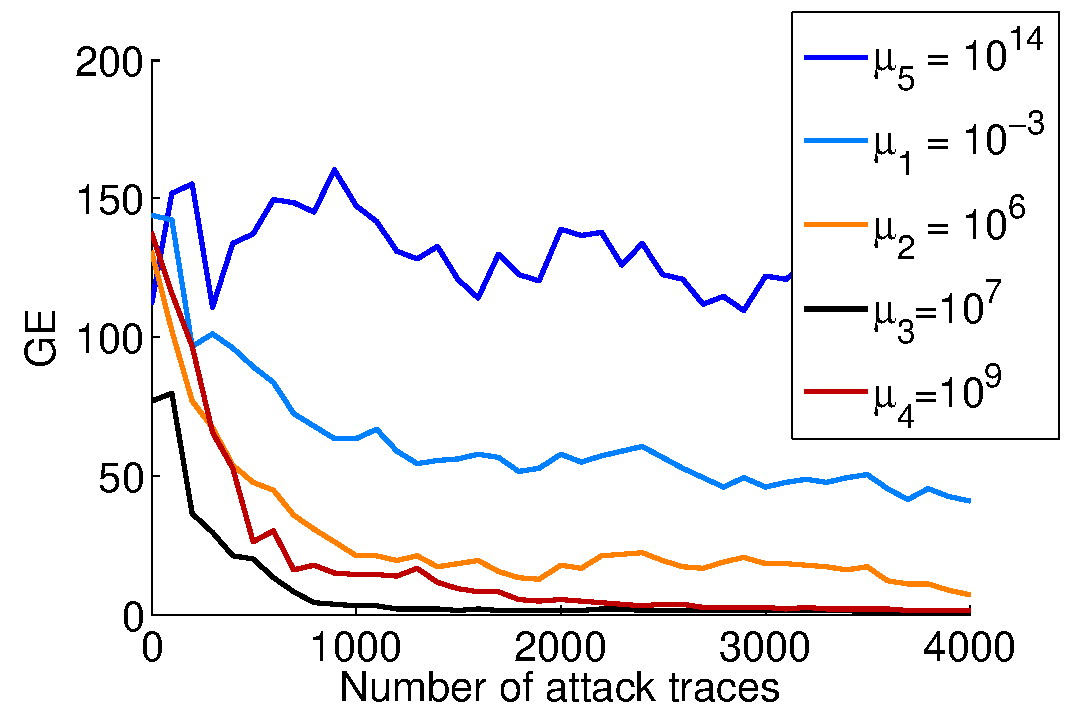
\includegraphics[width=.5\textwidth]{../Figures/CARDIS2016/mu_comparison_new.pdf} 
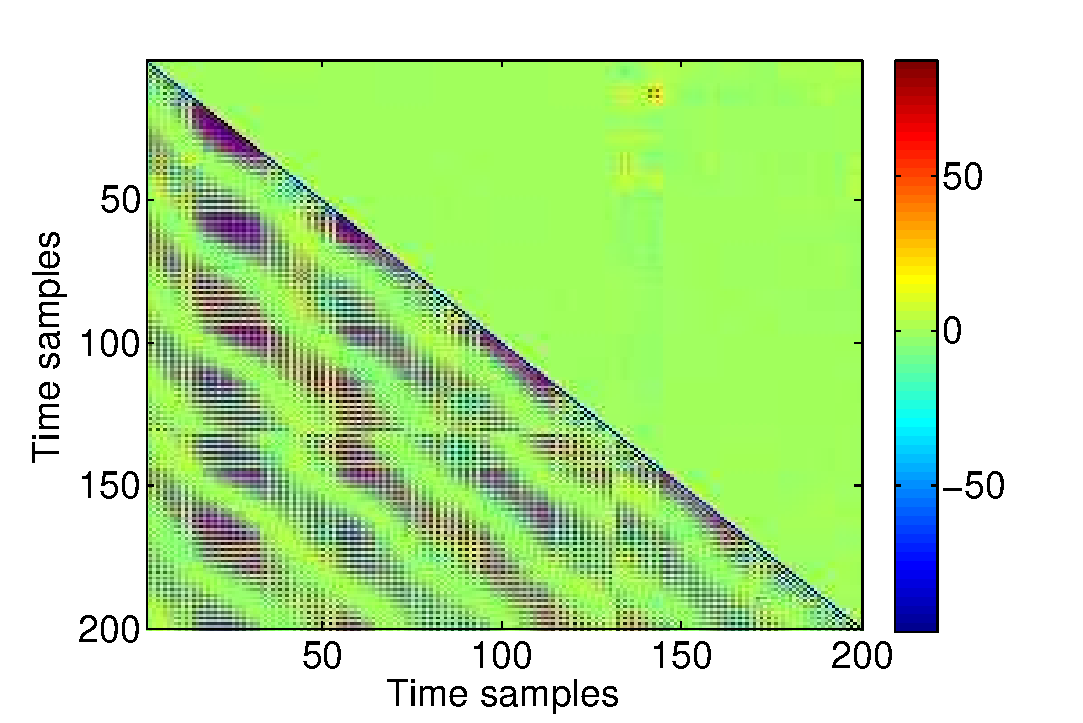
\includegraphics[width=.5\textwidth]{../Figures/CARDIS2016/good_bad_coeffs.pdf} 
\caption[Dependence of KDA performances on the regularization parameter $\mu$. Implicit coefficients.]{On the left: template attack guessing entropy vs the number of traces for the attack phase, varying for choices of the constant $\mu$  \eqref{eq:mu}. On the right: the implicit coefficients assigned to pairs of time samples for $\mu_3$ (upper triangular part) and $\mu_5$ (lower triangular part). }\label{fig:mu}
\end{figure}


By construction the matrix $\NNN$ in \eqref{eq:N} is not positive-definite, which is one of the reasons why \cite{scholkopf1999fisher} proposes the regularization \eqref{eq:mu} recalled hereafter:
\begin{equation}
\NNN = \NNN + \mu\III \mbox{ .}
\end{equation}

When applying such a regularization, the choice of the constant $\mu$ is crucial. For sure it has to be large enough to ensure that $\NNN$ turns to a positive-definite matrix, but we experimentally observed  that the minimal $\mu$ for which the positive-definitiveness of $\NNN$ is attained is often far from  being the one that provides a good extractor. In Fig.~\ref{fig:mu} (left) we observe the efficiency of a template attack run in combination with a KDA extractor. The matrix $\NNN$ is positive-definite for $\mu_1 = 10^{-3}$ but the value that provides the best extractor is much higher (namely $\mu_3 = 10^{7}$). Still raising the value of $\mu$ degrades the quality of the extractor. The right part of Fig.~\ref{fig:mu} shows the implicit coefficients of the extractor (see \eqref{eq:implicit}) obtained under $\mu_3$ (upper triangular part) and under $\mu_5$ (lower triangular part). The extractor corresponding to the former one leads to a successful attack and has high values concentrated over the interesting windows; the extractor corresponding to the latter one leads to an unsuccessful attack and shows lack of localization around interesting parts of the trace, highlighting the fact that the KDA tool failed in detecting generalisable class-distinguishing features in this case.\\

The regularization \eqref{eq:mu} is a proper regularization in the sense discussed in Sec.~\ref{sec:overfitting}: it is not only a way to make the problem computationally stable (which explains why the minimal $\mu$ making $\NNN$ positive-definite may not be a good choice), but also a answer to the overfitting phenomenon. In the case of the KDA the overfitting is observable when $\extract^{\mathrm{KDA}}$ almost perfectly separates the training traces in their classes, while failing in separating the attack ones. As explained in \cite{scholkopf1999fisher}, the regularization \eqref{eq:mu} corresponds to the additional requirement for $\nununu$ to have a small norm $\lVert\nununu\rVert^2$. As any regularization technique, it makes the method less accurate in the learning phase, but in some cases more likely to correctly operate on new examples.

\begin{remark}
Another regularization strategy may be to search for sparse vectors of implicit coefficients (see \eqref{eq:implicit}). This alternative might be more suitable for the side-channel context, since it would promote localized solutions, \emph{i.e.} projections for which only a few $d$-tuples of time samples contribute to the construction of the extractor (see Chapter~\ref{ChapterLinear} for an analogy in $1st$-order context). This approach is left for future developments.
\end{remark} 


Some heuristics exist to choose the constant $\mu$; {\em e.g.} the average of the diagonal entries \cite{multiclassLDA} or the minimal constant that let $\NNN$ be diagonally dominant (implying positive-definite), etc. In \cite{centeno2006optimising} Centeno \emph{et al.} propose a maximization strategy to find the optimal regularization parameter, based on a probabilistic approach. The study of this approach is left for future works. For our study we simply performed experiments for various values of $\mu$ and we kept the best obtained results.

\begin{remark}\label{rem:mu_criteria}
A criterion to decide whether the chosen regularization is convenient consists in comparing the SNR computed over the extracted training traces $(\extract^{\mathrm{KDA}}(\vLeakVec_i))_{i=1,\dots,\nbProfilingTraces}$ with the one computed over some extracted new traces $\yyy_i$ (\emph{e.g.} the profiling traces $(\extract^{\mathrm{KDA}}(\yyy_i))_{i=1,\dots,\nbProfilingTraces}$). If the latter is significantly lower than the former, the regularization failed and it is worth to try with another constant$\mu$.
\end{remark}


\subsection{The Multi-Class Trade-Off}\label{sec:multiclass}

\begin{figure}[t]
\subfigure[]{\label{fig:numClasses-2order}
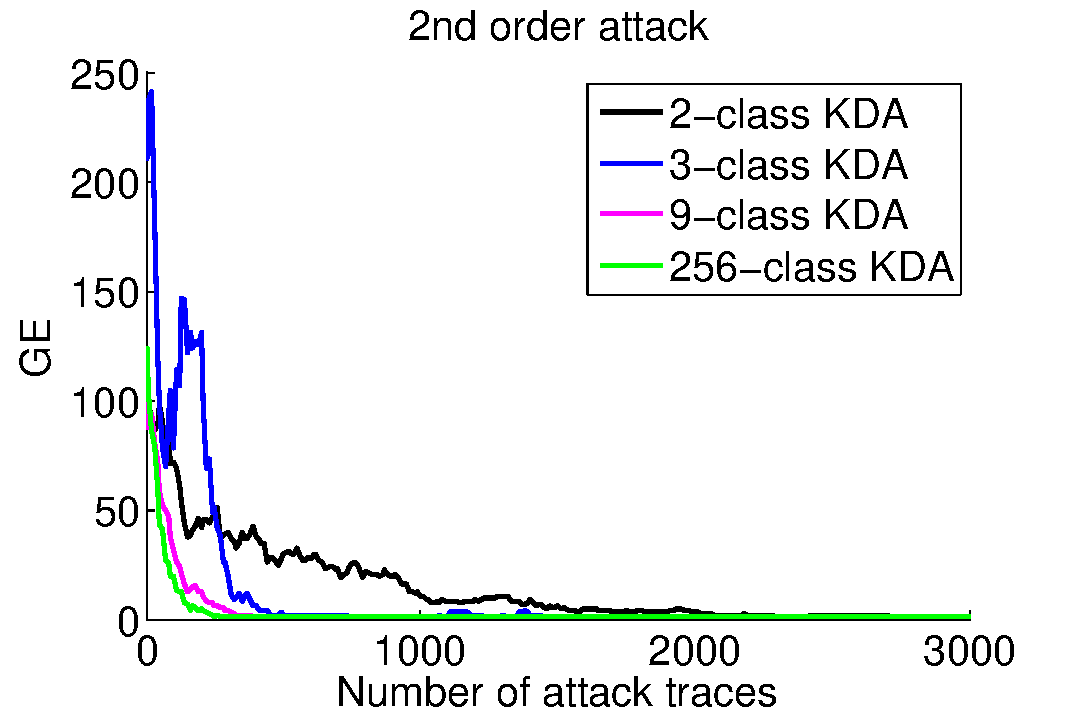
\includegraphics[width=.5\textwidth]{../Figures/CARDIS2016/2order_classes_TA.pdf}}
\subfigure[]{\label{fig:numClasses-3order}
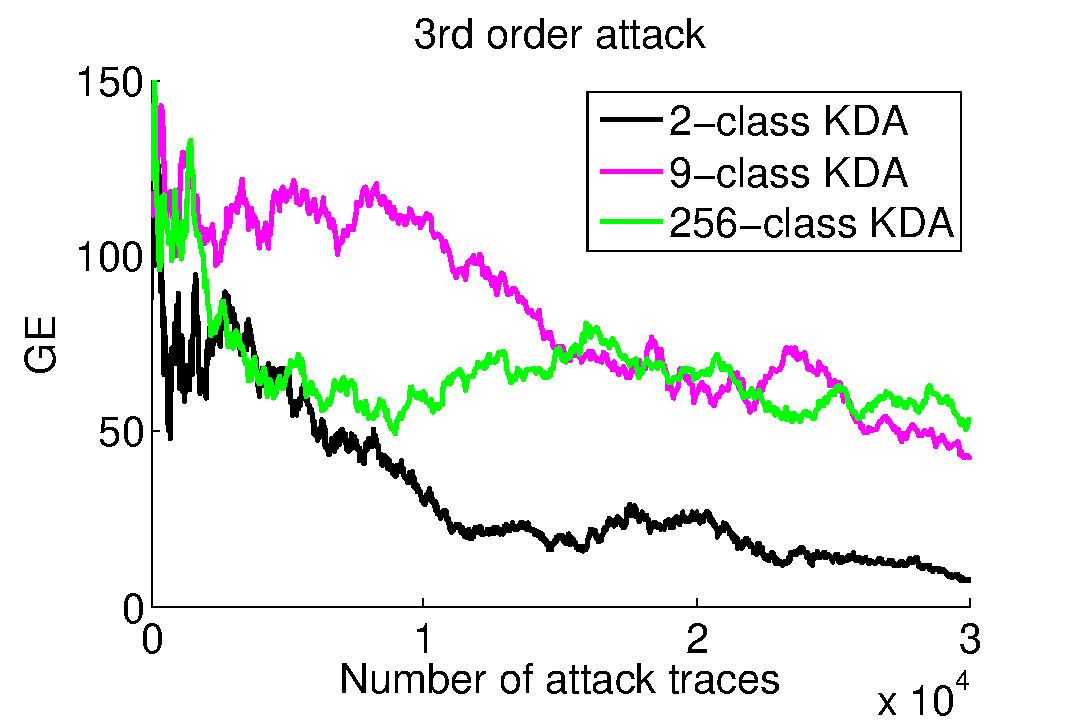
\includegraphics[width=.5\textwidth]{../Figures/CARDIS2016/3order_new.pdf}}
\caption[Comparison between 2-class,3-class, 9-class and 256-class KDA.]{Comparison between 2-class,3-class, 9-class and 256-class KDA in $2$nd-order context \subref{fig:numClasses-2order} and in $3$rd-order context \subref{fig:numClasses-3order}. For $2$nd-order the KDA is efficient in providing separability between 256 classes, allowing an optimal attack. In $3$rd-order context the training data are not enough to succeed the 256-class learning phase. Decreasing the number of classes to be distinguished raises the efficiency of the learning problem and thus of the attack.}\label{fig:numClasses}
\end{figure}

As discussed in Sec.~\ref{sec:LDA}, the LDA, and by consequence the KDA, looks for a subspace of the feature space to optimally separate some given classes (for a well-chosen distance). Intuitively the more examples( \emph{i.e.} training traces) available the more accurate the resulting KDA. Nevertheless, the number of examples might be bounded by the acquisition context. Actually even when the number $\nbProfilingTraces$ can be very high, it may be interesting to minimize it since the KDA complexity is $O(\nbProfilingTraces^3)$. A trade-off must therefore be found between accuracy and efficiency. Assuming that the size of the training set  is fixed to $\nbProfilingTraces$, which controls the efficiency, a way to gain in accuracy may be found by appropriately adjusting the number of classes to distinguish: again intuitively, the more examples per class, the more accurate the detection of a separating subspace. Then, if the total number of training traces is fixed, in order to raise the number of traces per class, a smaller number of classes must be considered. To do so, a non-injective model $m(\cdot)$ can be introduced, to create a smaller set of labels $m(\sensVarSet)$ from the initial set $\sensVarSet$. In the rest of the paper, the reduced number of classes, \emph{i.e.} the number of labels assigned to the training set after applying the model $m$, will be denoted by $W$ (it is the cardinality of $m(\sensVarSet)$). In order to not corrupt the soundness of the KDA method in the SCA context, it is worth choosing a meaningful model. As discussed in Sec.~\ref{sec:leakage_model}, a widely-accepted power-consumption model for side-channel traces is provided by the Hamming Weight ($\HW$) function, it makes sense to group the different values of $\sensRandVar$ according to their Hamming weights. In Fig.~\ref{fig:numClasses} we compared a $2$-class model ($m(\sensVar) =0$ if $\HW(\sensVar)<4$, $m(\sensVar) =1$ if $\HW(\sensVar)\geq4$), a $3$-class model ($m(\sensVar) =0$ if $\HW(\sensVar)<4$, $m(z) =1$ if $\HW(\sensVar)=4$, $m(\sensVar) =2$ if $\HW(\sensVar)>4$) and a $9$-class one ($m(\sensVar)=\HW(\sensVar)$).


\begin{remark}
A balanced training set of size $\nbProfilingTraces=9000$ (instead of 8960) has been used to run the experiments for $2$-class, $3$-class and $9$-class KDA.
\end{remark}

\begin{remark}\label{rem:efficiency}
For the sake of consistency\footnote{A different approach is analysed in Sec.~\ref{sec:asymmetric}.} between the pre-processing phase and the attack phase, when a non-injective model is applied to the labels of the training set to reduce the number of classes, the same model is exploited to run the template attack: $W$ templates (one per each class) are computed and compared to the matching traces. Thus, in Fig.~\ref{fig:numClasses} the different multi-class extractors are compared using different template attacks. It may be remarked that as $W$ decreases the efficiency of the attack is supposed to decrease as well, because each attack trace contributes in distinguishing the right key $\keyRandVar^\star$ only from a growing-size set of indistinguishable hypotheses. 
\end{remark}

In $2$nd-order context, it can be observed in Fig.~\ref{fig:numClasses} that the KDA is provided with sufficient training traces to succeed a 256-class separation, which allows the finest characterization of the leakage, and leads as expected (see Remark~\ref{rem:efficiency}), to the most efficient template attack. Moving to the $3$-rd order context, the available training set is insufficient to make the multi-class approach succeed; nevertheless, turning the problem into a 2-class problem turns out to be a good strategy to trade extraction accuracy for attack efficiency.



\begin{remark}\label{rem:numComp}
The separating subspace given by the KDA has maximal dimension $(W-1)$, \emph{i.e.} $Q\leq (W-1)$ in point 4 of Procedure~\ref{procedure:KDA}. When $W=2$ a single discriminant component $\extract^{\mathrm{KDA}}_1$ is available, then we run a univariate template attack, instead of a bivariate one. 
\end{remark}


\begin{figure}
\centering
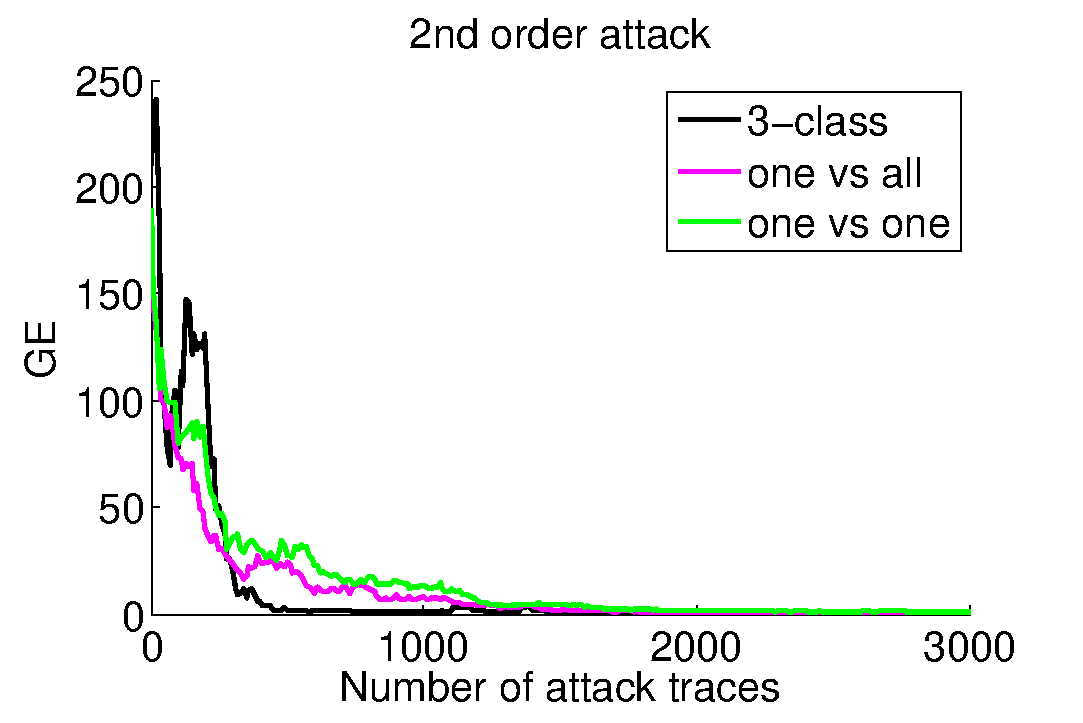
\includegraphics[width=.5\textwidth]{../Figures/CARDIS2016/2order_MULT.pdf}
\caption[KDA: comparison between multi-class, one vs one and one vs all approaches.]{Performance of template attacks run over 3-class KDA subspaces: multi-class, one vs one and one vs all approaches compared.}\label{fig:3multi-class}
\end{figure}

An idea to avoid an excessive reduction of the number of separable classes $W$ can be found in the machine learning literature dealing with the so-called \emph{multi-class classification problems}. It consists in treating the $W$-class problem as  multiple 2-class problems. Two different \emph{modus operandi} exist: the \emph{one-vs-one} and the \emph{one-vs-all}. When applied to our context, the one-vs-one approach determines for each pair of classes the 1-dimensional subspace that best separates them and exploits all the obtained subspaces to run an attack (for $W$ classes we obtain ${W}\choose{2}$ dimensions and we run a ${W}\choose{2}$-variate template attack). The one-vs-all approach looks for dimensions that best separate each class from all the others (obtaining $W$ projections in total).\\


We tested this approach in the 3-class case: in this way the one-vs-one and the one-vs-all approaches provide both 3 dimensions that we use to run a $3$-variate template attack, and that we compare to the $3$-class multi-class approach with bivariate template attack. Our experimental results, summed up in Fig.~\ref{fig:3multi-class}, show that no gain  is obtained by the 2-classes strategies.\footnote{We think that is result is quite data-dependant, so the use of such an approach is not discouraged in general.} We therefore chose to not consider them for our higher-order experiments.



\subsection{Asymmetric Preprocessing/Attack Approach}\label{sec:asymmetric}

\begin{figure}
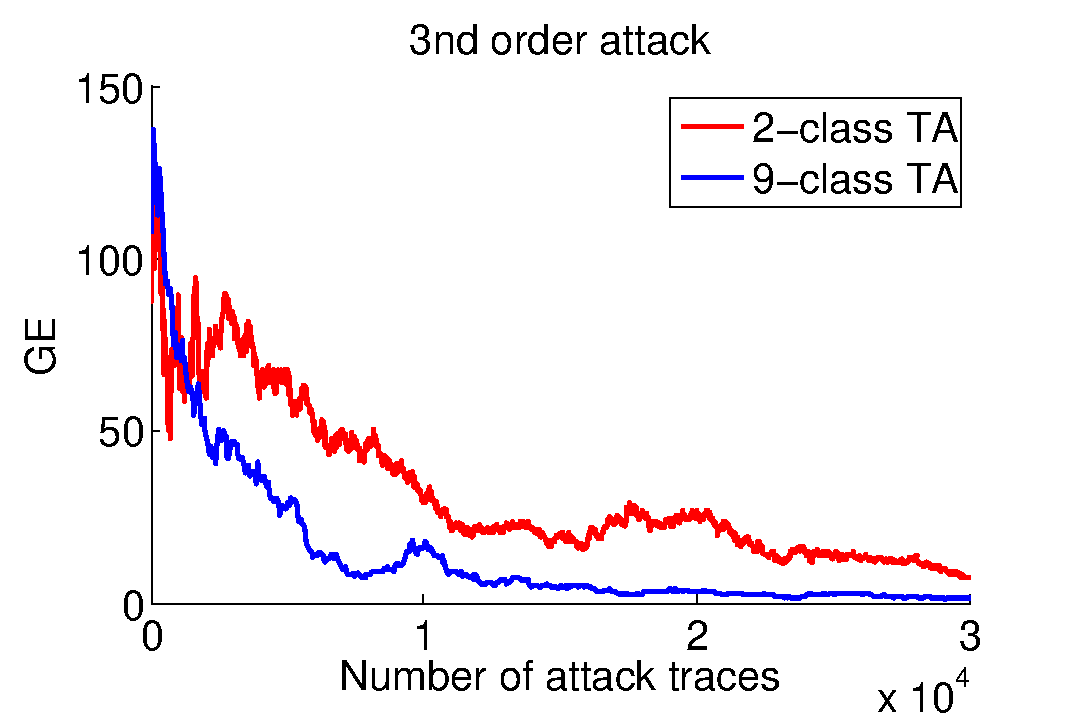
\includegraphics[width=.5\textwidth]{../Figures/CARDIS2016/3order_2_9.pdf} 
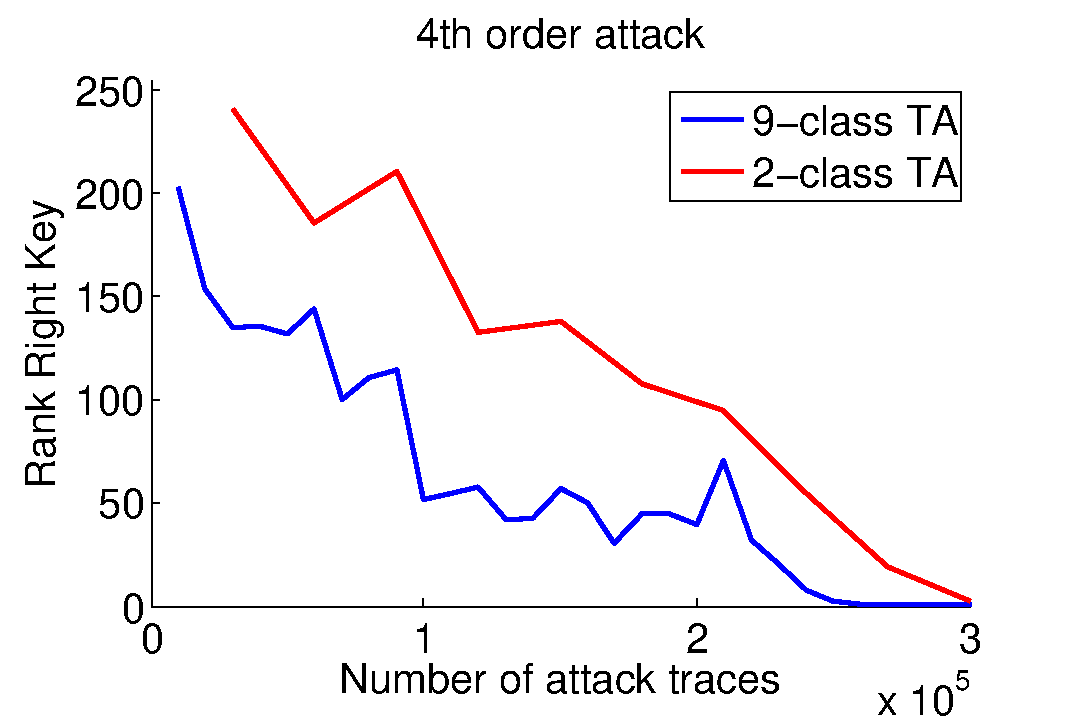
\includegraphics[width=.5\textwidth]{../Figures/CARDIS2016/4order_2_9.pdf} 
\caption[KDA preprocessing performance for  $3$rd-order and $4$th-order template attack]{Left: guessing entropy (over 10 independent tests) for a 2-class and a 9-class $3$rd-order template attack. Right: right key rank of a 2-class and a 9-class $4$th-order template attack.}\label{fig:3-4}
\end{figure}
In Remark~\ref{rem:efficiency} we appealed a consistency principle to justify the choice of running a $W$-class template attack after a $W$-class KDA extraction. Here we propose a different reasoning: the consistency principle does not grant that an extractor $\extract^{\mathrm{KDA}}$ trained with $W$ classes is not able to separate $W^\prime$ classes with $W^\prime > W$. As seen in Remark~\ref{rem:implicit}, an extractor $\extract^{\mathrm{KDA}}$ always implicitly performs a weighed sum, via the implicit coefficients, of centred products of time samples. If $\extract^{\mathrm{KDA}}$ is effective, the implicit coefficients which have the highest magnitude must correspond to time samples corresponding to the manipulation of sensitive data (\emph{e.g.} the variable shares when masking is applied). This property is not necessarily related to the number of classes used to train the the extractor.\\

Based on the reasoning above and on the observations reported in Remark \ref{rem:efficiency}, we performed in $3$rd-order and $4$th-order contexts a $9$-class template attack after the $2$-class KDA preprocessing.  The results are depicted in Fig.~\ref{fig:3-4} and confirm that, for our experimental data, this approach is sound: in both cases, using the same extractor trained with 2 classes and the same attack traces, the $9$-class approach outperforms the $2$-class one.
 
\begin{remark}
We choose to run the $9$-class instead of the $256$-class template attack in order to raise the accuracy of the profiling phase, being limited in terms of profiling traces. 
\end{remark}


\subsubsection{Comparison with Projection Pursuits}\label{sec:comparisonPP}

To get a fair comparison, we run the PP algorithm (see Sec.~\ref{sec:PP_description}) over the same training set used to evaluate the KDA in Sec.\ref{sec:practice}. The best results in the $2$nd-order context were obtained with the HW model (\emph{i.e.}  $\lvert \sensVarSet \rvert=9$). In this case $T_{det}$ is fixed to $0.7$. Since 4 training sets are required, the 9000 training traces are split in 4 equally-sized groups.  Experimental observations allowed to fix  $W_{len}=5$, consequently suggesting $minWS=1$, $maxWS = 15$ and consistent global and local movements and resizes.
 Given the heuristic asset of the algorithm, we run it 1000 times for $d=2$ and for $d=3$. An overview of the global behaviour of the obtained results is depicted in Figs~\ref{fig:PP2} and \ref{fig:PP3}: the lower parts of the figures show the sum of the 1000 outputs of the algorithm.
  We recall that each coordinate of $\AAlpha$ is set to 1 for the windows identified to be of interest, and to 0 elsewhere, so for each time sample the sum of the values ($0$ or $1$) assigned by the $1000$ attempts give an intuition about its likelihood to be considered as interesting by the PP method. It can be observed that in the $2$-nd order case (Fig.~\ref{fig:PP2}) the results are excellent: 100\% of the tests highlight an informative part of the two clock-cycles where the sensitive shares are manipulated.\footnote{It can be observed that the regions selected by $\extract^{PP}$ correspond to those for which the $\extract^{KDA}$ exhibits the highest magnitude implicit coefficients (Fig.~\ref{fig:mu}, upper-triangular part on the right)}
It means that $\extract^{PP}(\vaLeakVec)$ always contains information about $\sensRandVar$ and a successful attack can be mounted over such extracted traces. The efficiency of such an attack depending on many factors, there is no interest in comparing it to the performances of the template attacks run in $2$nd-order context using $\extract^{KDA}$ and depicted in Fig.~\ref{fig:numClasses-2order}.
As it may be observed in Fig.~\ref{fig:PP3}, in the $3$-rd order case the experimental results are completely different: almost no $\AAlpha$ selects the clock-cycle where the second share is manipulated. Thus in this case the PP approach fails: $\extract^{PP}(\vaLeakVec)$ does not contain information about $\sensRandVar$, so any attack launched over the extracted traces would fail, while $\extract^{KDA}$ still allows successful attacks in $3$rd-order and $4$th-order case, as depicted in Fig.~\ref{fig:3-4}.\\

\begin{figure}[t]
\subfigure[]{\label{fig:PP2}
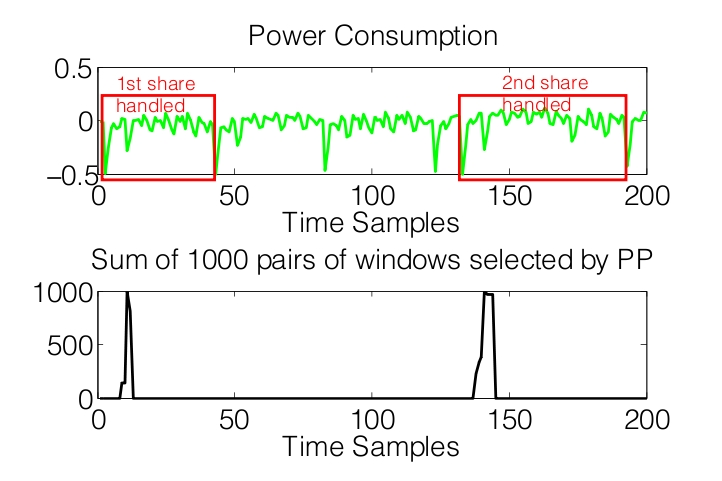
\includegraphics[width=.5\textwidth]{../Figures/CARDIS2016/secondOrderPP_gimp.jpg}}
\subfigure[]{\label{fig:PP3}
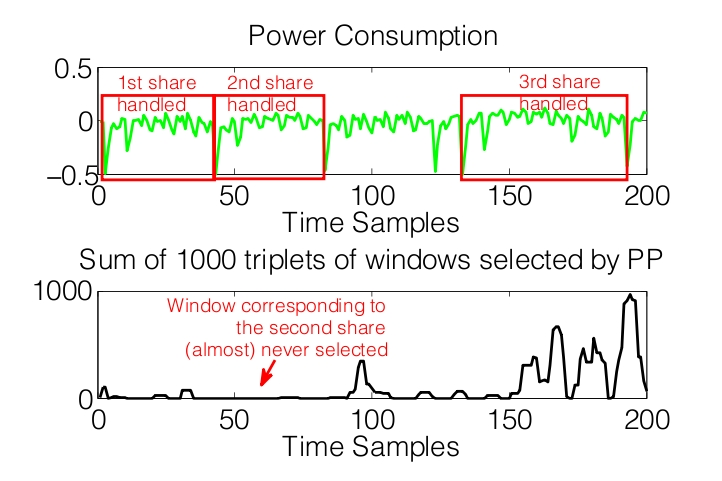
\includegraphics[width=.5\textwidth]{../Figures/CARDIS2016/thirdOrderPP_gimp.jpg}}
\caption[Overview of Projection Pursuit outputs in $2$nd-order and $3$rd-order context.]{\subref{fig:PP2} Overview of PP outputs in $2$nd-order context. \subref{fig:PP3} Overview of PP outputs in $3$rd-order context. }
\end{figure}

We conclude that the KDA approach is a valuable alternative to the PP one, especially in contexts where the training set size is bounded and independent from the order $d$ of the attack.


%----------------------------------------------------------------------------------------
%	SECTION 5
%----------------------------------------------------------------------------------------
\section{Drawbacks of Kernel Methods}
\subsubsection{Misalignment Effects}
\subsubsection{Memory Complexity and Actual Number of Parameters}
\subsubsection{Two-Phases Approach: Preprocessing-Templates}
% che tra l'altro per farlo dividi le tracce di profilaggio in due

% Chapter Template

\chapter{Convolutional Neural Networks against Jitter-Based Countermeasures} % Main chapter title

\label{ChapterCNN}
%----------------------------------------------------------------------------------------
%	SECTION 1
%----------------------------------------------------------------------------------------

\section{Moving from Kernel Machines to Neural Networks}
% The answers to the 3 drawbacks of previous chapter (misalignment, memory complexity and actual number of params, two phases approach)
%"In practice, however, it is often worth investing substantial computational resources during the training phase in order to obtain a compact model that is fast at processing new data" (Bishop intro chap 5)
\subsection{Multi-Layer Perceptrons}
% descrizione (dal paper) 
% universal approximation theorem (da pagg 194 e seguenti del deeplearningbook)

%----------------------------------------------------------------------------------------
%	SECTION 2
%----------------------------------------------------------------------------------------

\section{Misalignment of Side-Channel Traces}

\subsection{The Necessity and the Risks of Applying Realignment Techniques}
\subsection{Analogy with Image Recognition Issues}

%----------------------------------------------------------------------------------------
%	SECTION 3
%----------------------------------------------------------------------------------------

\section{Convolutional Layers to Impose Shift-Invariance}

%----------------------------------------------------------------------------------------
%	SECTION 4
%----------------------------------------------------------------------------------------

\section{Data Augmentation for Misaligned Side-Channel Traces}
\todo{cita o qui o all'inizio il paper di CARDIS 2017 sulla trace augmentation}
%----------------------------------------------------------------------------------------
%	SECTION 5
%----------------------------------------------------------------------------------------

\section{Experiments against Software Countermeasures}


%----------------------------------------------------------------------------------------
%	SECTION 6
%----------------------------------------------------------------------------------------

\section{Experiments against Artificial Hardware Countermeasures}\label{sec:hardware}%label citato in appendice artifical jitter

%----------------------------------------------------------------------------------------
%	SECTION 7
%----------------------------------------------------------------------------------------

\section{Experiments against Real-Case Hardware Countermeasures}

% Chapter Template

\chapter{Conclusions and Perspectives} % Main chapter title

\label{ChapterConclusions}

% use bayesian inference with 'key' as parameter (usa la chiave esplicitamente come parametro e ogni volta che aggiungi una traccia, aggiorna le distribuzioni a priori della variabile sensibile per calcolare la likelihood...)

%----------------------------------------------------------------------------------------
%	SECTION 1
%----------------------------------------------------------------------------------------

\section{Summary}

%----------------------------------------------------------------------------------------
%	SECTION 2
%----------------------------------------------------------------------------------------

\section{Strengthen Embedded Security: the Main Challenge for Machine Learning Applications}

%----------------------------------------------------------------------------------------
%	THESIS CONTENT - APPENDICES
%----------------------------------------------------------------------------------------

\appendix % Cue to tell LaTeX that the following "chapters" are Appendices


%\chapter{Scenario 3 and 4 of CARDIS '15 paper}\label{Appendix_scenario3_4_cardis2015}

\section{Scenario 3.}
Let  $\newTraceLength$ be now variable and let the other parameters be fixed as follows: $\nbAttackTraces = 100, N_z=200, \numPoI = 3996$. Looking at Fig.~\ref{fig:3}, we might observe that the standard PCA might actually well perform in SCA context if provided with a larger number of kept components; on the contrary, a little number of components suffices to the LDA. Finally, keeping more of the necessary components does not worsen the efficiency of the attack, which allows the attacker to choose $\newTraceLength$ as the maximum value supported by his computational means.

\begin{remark}
In our experiments the ELV selection method only slightly outperforms the IPR. Nevertheless, since it relies on more sound and more general observations, {\em i.e.} the maximization of explained variance concentrated into few points, it is likely to be more robust and less case-specific. For example, in Fig.~\ref{fig:notSSS} it can be remarked that while the class-oriented PCA + ELV line keeps constant on the value 0 of guessing entropy, the class-oriented PCA + IPR is sometimes higher than 0.
\end{remark}

\todo{Is the table with results overview interesting?}
%
%\medskip
%
%\medskip
%
%  \begin{minipage}[c]{\textwidth}
%  \hspace*{-3mm}
%  \begin{minipage}[c]{0.45\textwidth}
%    \centering
%    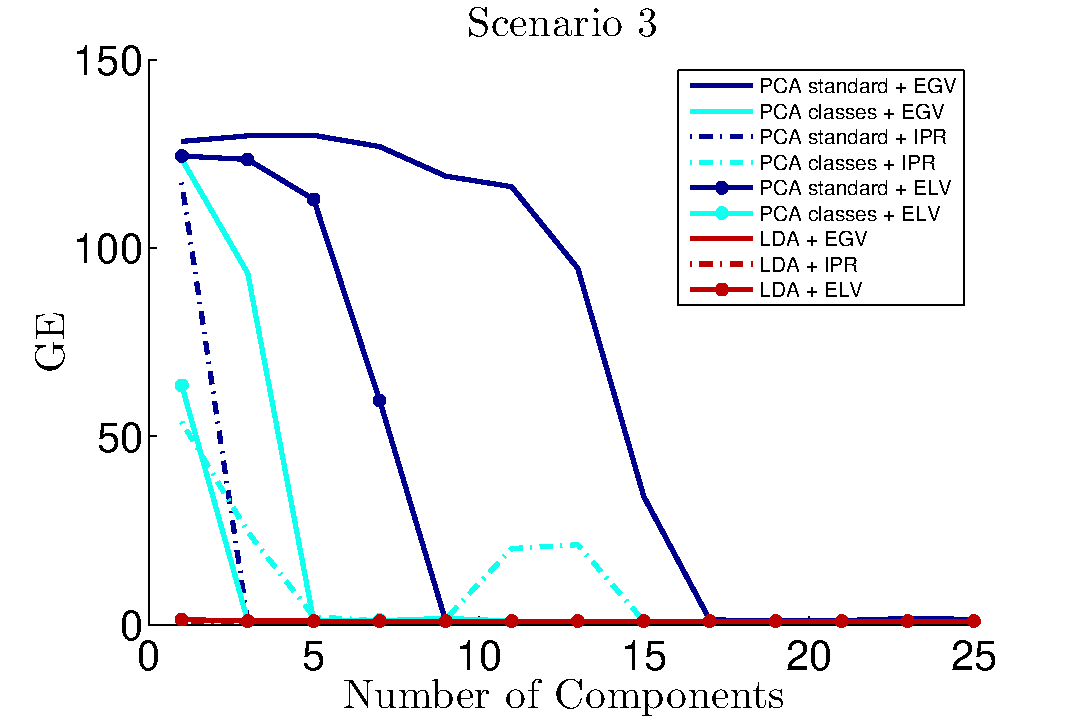
\includegraphics[width=\textwidth]{figures/Criterion3.pdf}
%    \captionof{figure}{Guessing Entropy as function of the number of the traces size after reduction}\label{fig:3}
%  \end{minipage}
%\hspace{1mm}
%  \begin{minipage}[c]{0.45\textwidth}
%    \centering
%    \begin{tiny}
%\begin{tabular}{|c|c|c|c|c|c|}
%\hline
%&&\multicolumn{4}{|>{\columncolor[gray]{0.7}}c|}{Parameter to minimize}\\
%\hline
%\multicolumn{1}{|>{\columncolor[gray]{0.7}}c|}{Method}&\multicolumn{1}{|>{\columncolor[gray]{0.7}}c|}{Selection}& $N$ &  $N'$ (SSS) &  $N'$ ($\neg$SSS) &  $C$ \\
%\hline
%PCA standard & EGV & {\bf -} &  &{\bf -} &{\bf -} \\
%\hline
%PCA standard &\multicolumn{1}{|>{\columncolor[gray]{0.8}}c|}{ELV} & \multicolumn{1}{|>{\columncolor[gray]{0.9}}c|}{{\bf -}} & &\multicolumn{1}{|>{\columncolor[gray]{0.9}}c|}{{\bf -}} &\multicolumn{1}{|>{\columncolor[gray]{0.9}}c|}{{\bf -}} \\
%\hline
%PCA standard & IPR &{\bf -} & &{\bf -} &{\bf +} \\
%\hline
%PCA class & EGV & {\bf -} &{\bf -} &{\bf -} &{\bf -} \\
%\hline
%PCA class & \multicolumn{1}{|>{\columncolor[gray]{0.8}}c|}{ELV} &\multicolumn{1}{|>{\columncolor[gray]{0.9}}c|}{{\bf +}} &\multicolumn{1}{|>{\columncolor[gray]{0.9}}c|}{$\bigstar$}&\multicolumn{1}{|>{\columncolor[gray]{0.9}}c|}{$\bigstar$} &\multicolumn{1}{|>{\columncolor[gray]{0.9}}c|}{{\bf +}} \\
%\hline 
%PCA class & IPR & {\bf {\bf +}} &$\bigstar$ &{\bf +} &{\bf -} \\
%\hline 
%LDA & EGV &$\bigstar$ & & {\bf +} & $\bigstar$\\
%\hline 
%LDA & \multicolumn{1}{|>{\columncolor[gray]{0.8}}c|}{ELV} & \multicolumn{1}{|>{\columncolor[gray]{0.9}}c|}{{\bf +}} &  & \multicolumn{1}{|>{\columncolor[gray]{0.9}}c|}{{\bf +}} & \multicolumn{1}{|>{\columncolor[gray]{0.9}}c|}{$\bigstar$}\\
%\hline 
%LDA & IPR & {\bf +} & &{\bf +} & $\bigstar$ \\
%
%\hline 
%\multicolumn{1}{|>{\columncolor[gray]{0.8}}c|}{$\SW$ Null Space}  & EGV & &\multicolumn{1}{|>{\columncolor[gray]{0.9}}c|}{$\bigstar$ } & & \\
%\hline 
%\multicolumn{1}{|>{\columncolor[gray]{0.8}}c|}{$\SW$ Null Space}  & IPR & &\multicolumn{1}{|>{\columncolor[gray]{0.9}}c|}{{\bf +}} & & \\
%\hline 
%\multicolumn{1}{|>{\columncolor[gray]{0.8}}c|}{Direct LDA} & EGV & & \multicolumn{1}{|>{\columncolor[gray]{0.9}}c|}{$\bigstar$}& & \\
%\hline 
%\multicolumn{1}{|>{\columncolor[gray]{0.8}}c|}{Direct LDA} & IPR & &\multicolumn{1}{|>{\columncolor[gray]{0.9}}c|}{{\bf +}}& & \\
%\hline
%\multicolumn{2}{|>{\columncolor[gray]{0.8}}c|}{Fisherface} & &\multicolumn{1}{|>{\columncolor[gray]{0.9}}c|}{{\bf -}} & & \\
%\hline 
%\multicolumn{2}{|>{\columncolor[gray]{0.8}}c|}{$\ST$ Spanned Space}  & &\multicolumn{1}{|>{\columncolor[gray]{0.9}}c|}{{\bf -}} & & \\
%\hline
%\end{tabular}
%\end{tiny}
%\captionof{table}{Overview of extractors performances in tested situations.}\label{table:results}
%    \end{minipage}
%  \end{minipage}
%
%\begin{figure}
%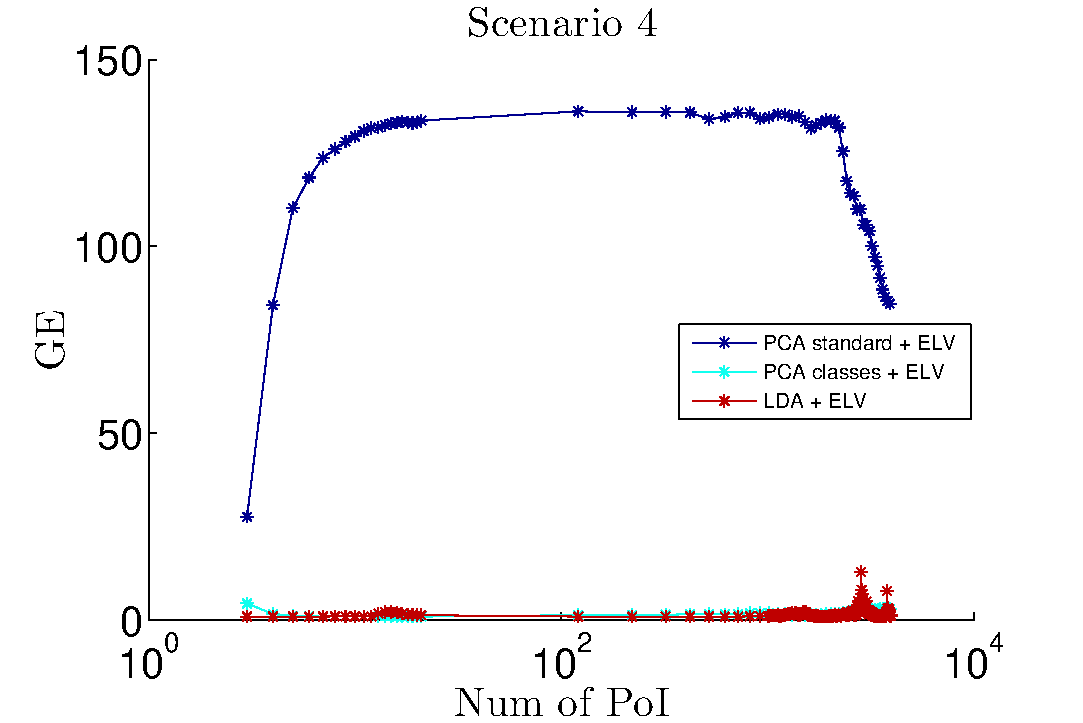
\includegraphics[width=0.5\textwidth]{figures/Criterion4.pdf}
%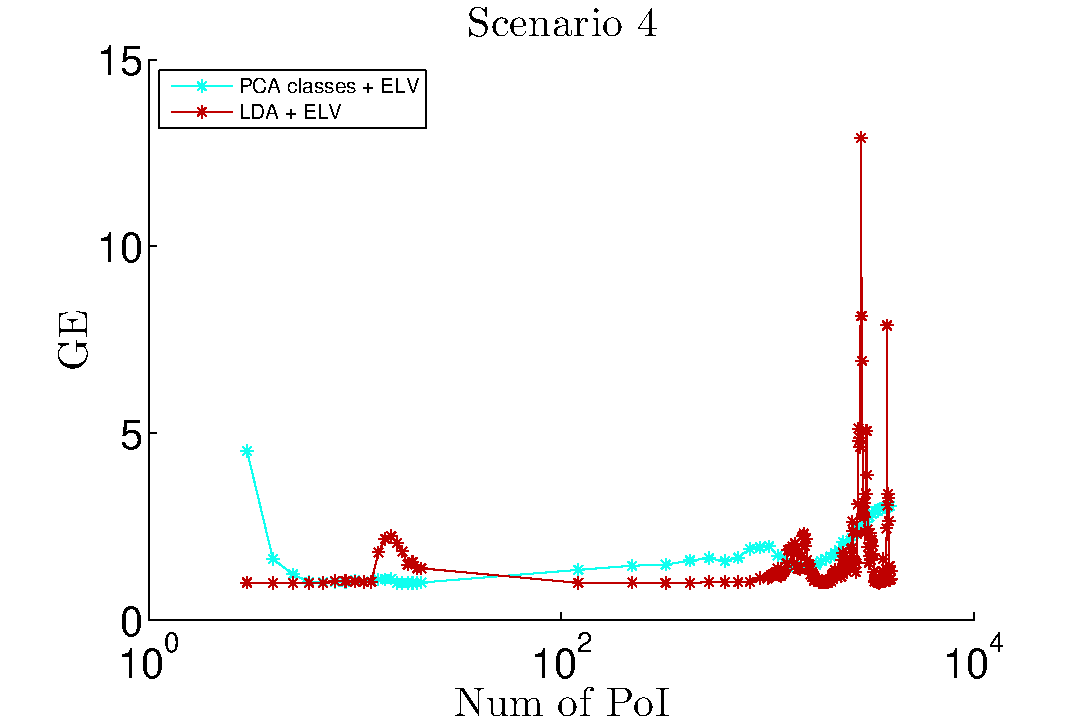
\includegraphics[width=0.5\textwidth]{figures/Criterion4cutted.pdf} 
%\caption{Guessing Entropy as function of the number of time samples contributing to the extractor computation.}\label{fig:4}
%\end{figure}
%
%An overview of the results of our comparison in scenarios 1, 2 and 3 is depicted in Table~\ref{table:results}: depending on the adversary purpose, given by the parameter to minimize, a $\bigstar$ denotes the best method, a ${\bf +}$ denotes a method with performances close to those of the best one and a ${\bf -}$ is for methods that show lower performances. Techniques introduced in this paper are highlighted by a grey background.  For example we remark that the class-oriented PCA takes advantage of the association with our ELV selection of components, achieving optimal performances when the goal is to minimize the number of profiling traces $\numTraces[]'$. As expected, when there are no constraints over $\numTraces[]'$, the LDA outperforms the other methods; however, even in this case which is very favourable to the LDA, the class-oriented PCA equipped with the ELV selection has an efficiency which is close to that of the LDA.
%


\section{Scenario 4.}


This is the single scenario in which we allow the ELV selection method to not only select the components to keep but also to modify them, keeping only some coefficients within each component, setting the other ones to zero. We select pairs \textit{(component, time sample)} in decreasing order of the ELV values, allowing the presence of only $\newTraceLength = 3$ components and $\numPoI$ different times samples: {\em i.e.}, we impose that the matrix $A$ defining the extractor (see \eqref{eq:linearExtractor}) has $\newTraceLength = 3$ rows (storing the 3 chosen components, transposed) and exactly $\numPoI$ non-zero columns.
Looking at Fig.~\ref{fig:4} we might observe that the LDA allows to achieve the maximal guessing entropy with only 1 PoI in each of the 3 selected components. 
Actually, adding PoIs worsen its performances, which is coherent with the assumption that the vulnerable information leaks in only a few points. Such points are excellently detected by the LDA. Adding contribution from other points raises the noise, which is then compensated by the contributions of further noisy points, in a very delicate balance. Such a behaviour is clearly visible in standard PCA case: the first 10 points considered raise the level of noise, that is then balanced by the last 1000 points.


\chapter{Cross-Validation} 

\label{app:cross-validation} 

In the ML community, several evaluation frameworks are commonly
applied to assess the performances of a model or to select the best hyper-parameters
for a learning algorithm. These methods aim to provide an
estimator of the performance which does not
depend on the choice of the training set $\setDataTrain$ (on which the model is trained) and of the
test set $\setDataTest$ (on which the model is tested) but only on their size.

The so-called \emph{$t$-fold
cross-validation} \cite{friedman2001elements} is currently the preferred evaluation method. Let P be a
performance metric, $\hat{f}$ a model to evaluate, and $\setDataTrain=(\setLeak, \setTarget)$ a labelled dataset, the outline of the method is the
following: 
\begin{enumerate}
\item ~[optional] randomize the order of the labelled traces in $\setDataTrain$, 
\item ~split the samples and their corresponding labels into $t$ disjoint parts
of equal size $(\setLeak_1,\setTarget_1),\ldots,(\setLeak_t,\setTarget_t)$.
For each $i\in [1..t]$, do:
\begin{enumerate}
\item set $\setDataValidation \doteq (\setLeak_i, \setTarget_i)$ and
$\setDataTrain \doteq (\bigcup_{j\neq i} \setLeak_j, \bigcup_{j\neq
i} \setTarget_j)$,
\item ~(re-)train\footnote{The model is trained from scratch at each iteration of the loop over $t$.} the model $\hat{f}$ on $\setDataTrain$, 
\item ~compute the performance metric $P_i$ by evaluating the model $\hat{f}$ on $\setDataValidation$,
%\begin{equation}\label{equ:perMetric}
%\text{P}_i = \text{P}(\hat{f}, \setDataValidation) \enspace ,
%\end{equation}
\end{enumerate}
\item ~return the mean $\frac{1}{t}\sum_{i=1}^t \text{P}_i$.
\end{enumerate}

It is known that the $t$-fold cross-validation estimator is an unbiased
estimator of the generalisation performance. Its main drawback is its variance
which may be large and difficult to estimate
\cite{breiman1996heuristics,bengio2005bias}. 
\chapter{Artificially Simulate Jitter}\label{appendix:artificial_jitter}

%\lstset{language=Python}

In order to analyse the behaviour of the techniques studied in this thesis over misaligned side-channel traces, we simulated sometimes a jitter effect to misalign some well-synchronized traces in a controlled way. When jittering is present, the clock stability is altered and clock cycles are sampled by a varying number of time samples. To simulate such effect, the windows containing clock patterns of an acquisition are selected one by one and passed as input to the following function, described in python code, in charge to enlarge or reduce them in a random way. The randomness depends on two parameters \texttt{sigma} and \texttt{B}, being the number of inserted or removed points be almost normally distributed, with standard deviation given by \texttt{sigma}, but bounded. The bound is controlled by \texttt{B} by the following rule: the final size of a window has to be at least $\frac{1}{\text{\texttt{B}}}$ times the original size and at most \texttt{B} times the original size. The value assigned to newly inserted points is the linear interpolation of the previous and the following points.

\begin{lstlisting}[frame=single]
def enlarge_reduce_window(window,sigma,B): 
    Npts = window.shape[0]
    new_window = np.copy(window)
    deltaPts = int(np.floor(np.random.randn(1)[0]*sigma))
    if (deltaPts >= 0):
        deltaPts = min(Npts*(B-1),deltaPts)
        for i  in range(deltaPts):
            curr_size = new_window.shape[0]
            pos = int(np.floor(np.random.rand(1)*curr_size))
            if pos==0 or pos==curr_size-1:
                new_window = np.insert(new_window,
                 pos,new_window[pos])
            else:
                new_window = np.insert(new_window,pos, 
                (new_window[pos-1]+
                new_window[pos])/2.0)
    else:
        deltaPts = max(-Npts*(1-1/B),deltaPts)
        for i in range(-deltaPts):
            curr_size = new_window.shape[0]
            pos = int(np.floor(np.random.rand(1)*curr_size))
            new_window = np.delete(new_window,pos)
    return new_window
    
\end{lstlisting}

This deformation is applied to each clock pattern independently. We remark that is implies that, for example, The 19th clock cycle of a deformed acquisition suffers from the cumulation of the previous 18 deformations. For the sake of visualizing the effect of such a jitter simulation, in Fig.~\ref{fig:jitter_traces} we depict some traces of  \emph{DS\_low\_jitter} \ref{fig:jitter_traces22} and of the \emph{DS\_high\_jitter} \ref{fig:jitter_traces66} datasets, used for experiments in Sec~.\ref{sec:hard}. They are obtained by perfectly synchronous acquisitions, with parameters set to \texttt{sigma} $= 2$, \texttt{B}$= 2$ for the \emph{DS\_low\_jitter}  dataset and \texttt{sigma} $= 6$, \texttt{B}$= 6$ for the \emph{DS\_high\_jitter} one.


\begin{figure}
\centering
\subfigure[]{\label{fig:jitter_traces22}
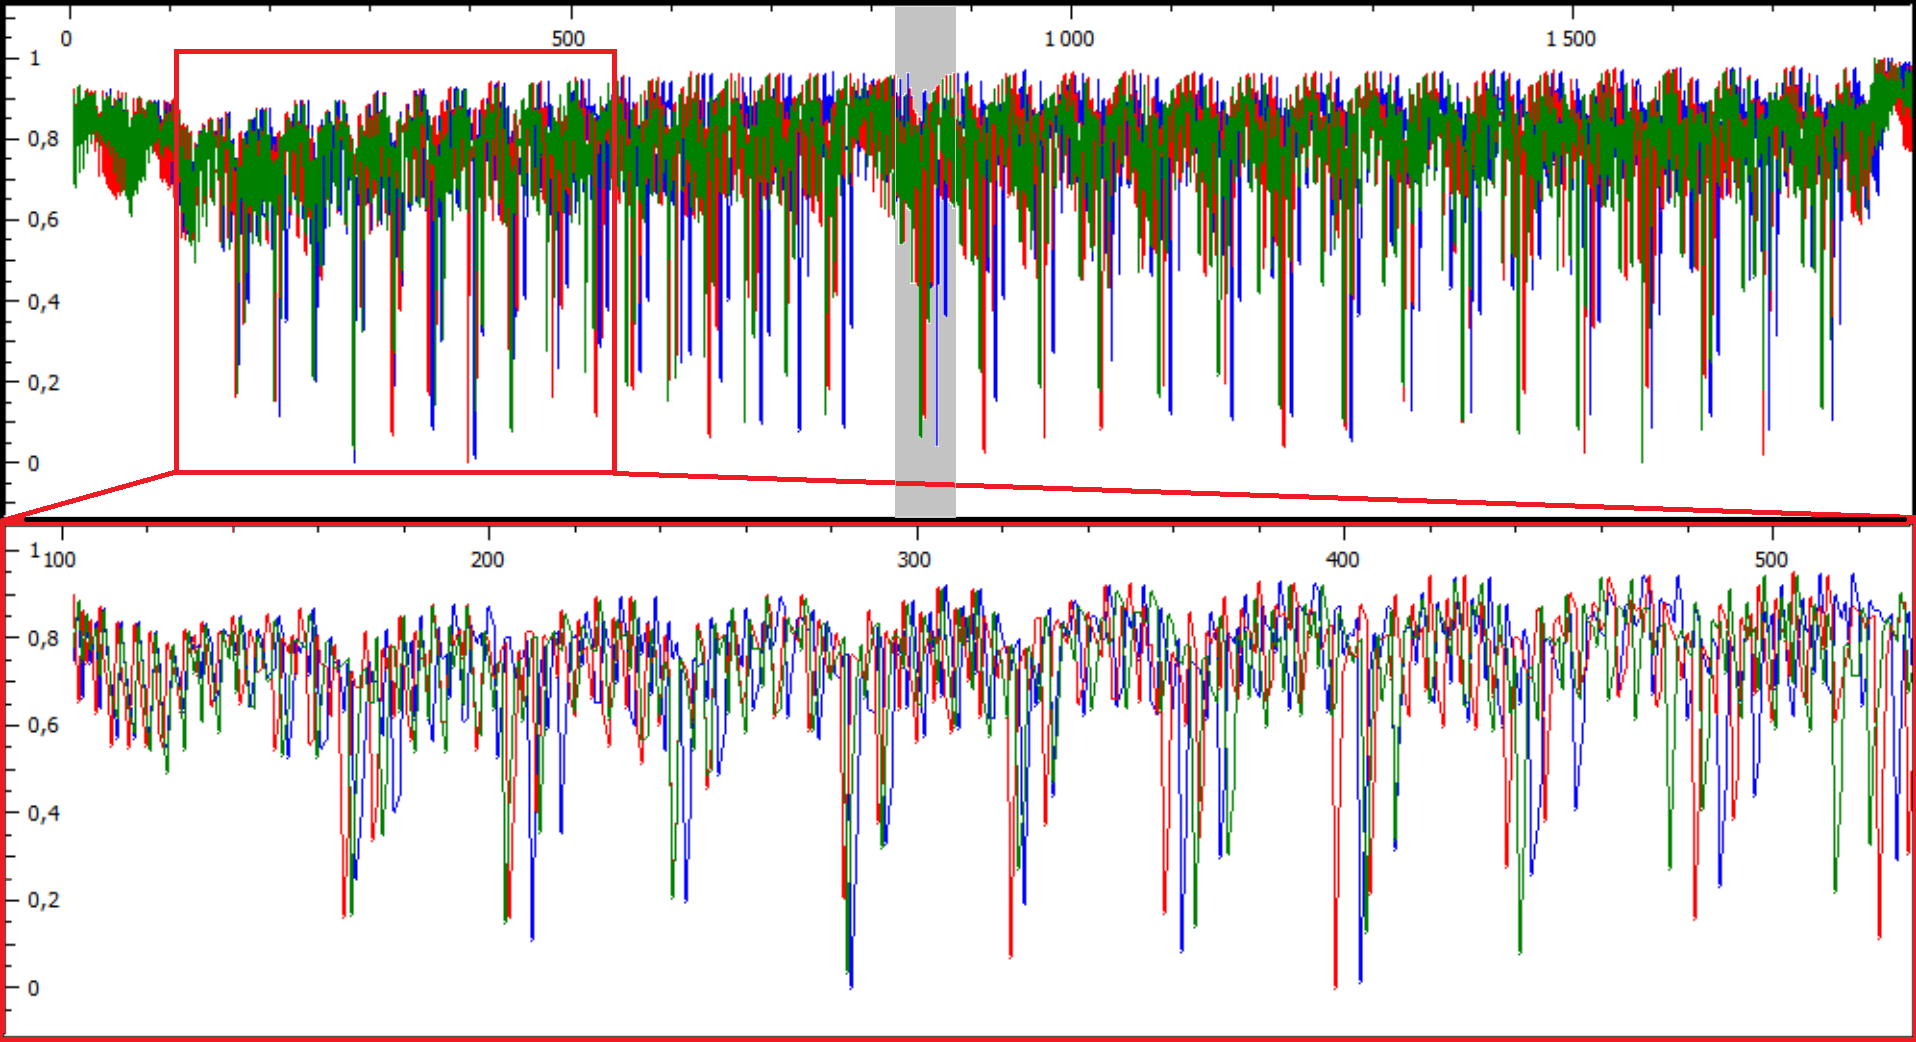
\includegraphics[width=\textwidth]{../Figures/CHES2017/jitter_2_2_framed.png} }
\subfigure[]{\label{fig:jitter_traces66}
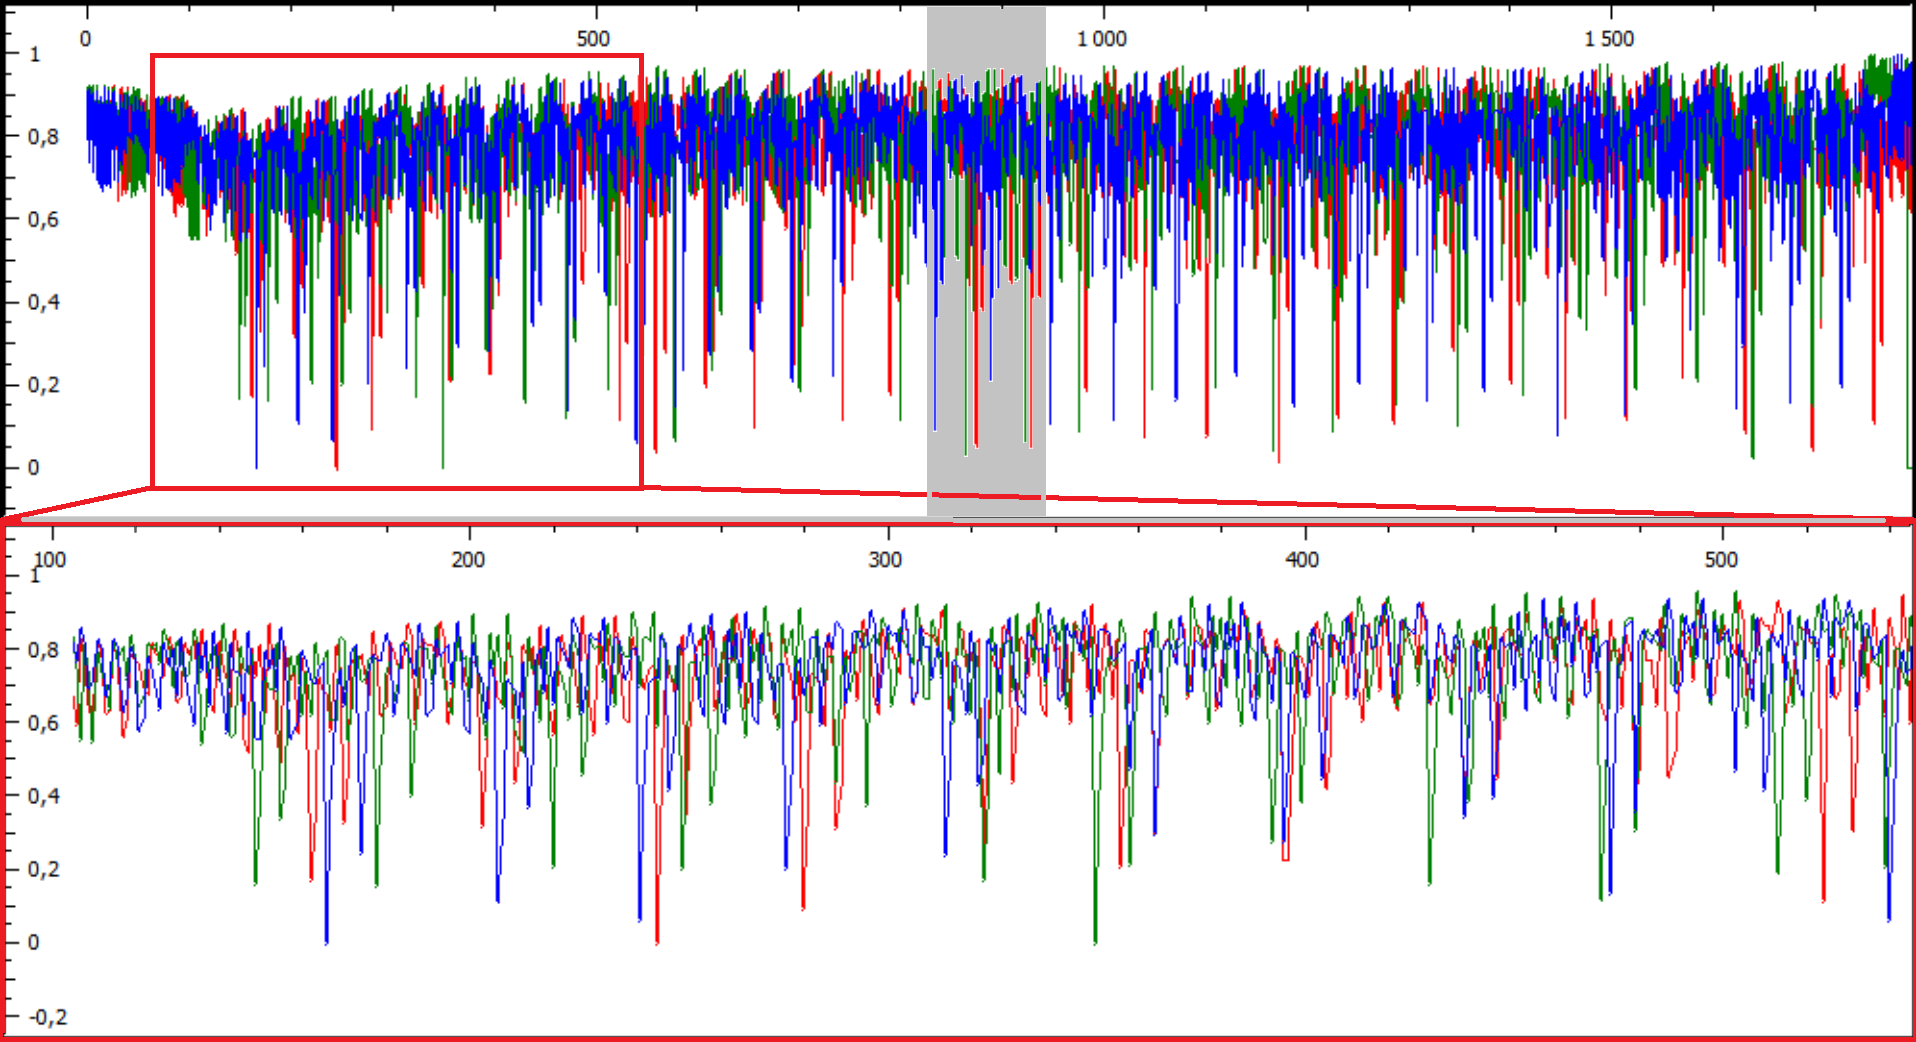
\includegraphics[width=\textwidth]{../Figures/CHES2017/jitter_6_6_framed.png} }
\caption[Hardware misalignment: \emph{DS\_low\_jitter} and \emph{DS\_high\_jitter} datasets.]{\subref{fig:jitter_traces22}  some traces of the \emph{DS\_low\_jitter} dataset, a zoom of the part highlighted by the red rectangle is given in the bottom part. \subref{fig:jitter_traces22} some traces of the \emph{DS\_high\_jitter} dataset. The interesting clock cycle is highlighted by the grey rectangular area.}\label{fig:jitter_traces}
\end{figure}


\chapter{Kernel PCA construction}\label{app:KPCA}

Suppose that we want to perform PCA in the image space of a function $\Phi$ that is associated to a given kernel function $K$. The kernel version for PCA has been presented in \cite{scholkopf1998nonlinear}, where all details can be found; as we said, the important step consists in expressing the operations needed for the PCA procedure in terms of the dot products between the mapped data.\\

Let us assume that data are centered in the feature space, {\em i.e.} $\sum_{i=1,\dots,\nbProfilingTraces}\Phi(\vLeakVec_{i})=0$.\footnote{Such a condition is not hard to achieve, even without explicitly pass through the feature space: it suffices substituting the kernel matrix $\kernelMatrix$ by the matrix $\tilde{\kernelMatrix} = \kernelMatrix - \boldsymbol{1}_{\nbProfilingTraces}\kernelMatrix - \kernelMatrix\boldsymbol{1}_{\nbProfilingTraces} + \boldsymbol{1}_{\nbProfilingTraces}\kernelMatrix\boldsymbol{1}_{\nbProfilingTraces}$, where $\boldsymbol{1}_{\nbProfilingTraces}$ denotes the matrix with each entry equal to $\frac{1}{\nbProfilingTraces}$. The same kind of matrix has to be computed in projecting phase, using the test data.} In this way the empirical covariance matrix $\covmat^\Phi$ of data in the feature space is given by:
\begin{equation}
\covmat^\Phi = \frac{1}{\nbProfilingTraces} \sum_{i=1}^{\nbProfilingTraces}\Phi(\vLeakVec_{i})\Phi(\vLeakVec_{i})^\intercal \mbox{ .}
\end{equation} 
We want to find eigenvalues $\lambda^\Phi \neq 0$ and eigenvectors $\AAlpha^\Phi\in \mathcal{F}\smallsetminus \{\boldsymbol{0}\}$ such that
\begin{equation}\label{eq:eigProblem}
\covmat^\Phi\AAlpha^\Phi = \lambda^\Phi \AAlpha^\Phi \mbox{ .}
\end{equation}
We remark that such an eigenvector satisfies
\begin{align}
\AAlpha^\Phi &= \frac{1}{\lambda^\Phi\nbProfilingTraces}\sum_{i=1}^{\nbProfilingTraces} \Phi(\vLeakVec_{i})\Phi(\vLeakVec_{i})^\intercal \AAlpha^\Phi\\
\label{eq:passaggio}
&=  \frac{1}{\lambda^\Phi\nbProfilingTraces}\sum_{i=1}^{\nbProfilingTraces} \left[\Phi(\vLeakVec_{i})^\intercal \AAlpha^\Phi\right] \Phi(\vLeakVec_{i}) =  \\
&= \sum_{i=1}^{\nbProfilingTraces}\underbrace{\frac{\Phi(\vLeakVec_{i})^\intercal \AAlpha^\Phi}{\lambda^\Phi\nbProfilingTraces}}_{\nu_i}\Phi(\vLeakVec_{i}) = \\
\label{eq:linearComb}
&= \sum_{i=1}^{\nbProfilingTraces}\nu_i \Phi(\vLeakVec_{i})\mbox{ ,}
\end{align}
where the step \eqref{eq:passaggio} makes use of the associativity of the matrix product and the commutativity of the scalar-matrix product. Eq.~\eqref{eq:linearComb} tells us that each eigenvector $\AAlpha^\Phi$ is expressible as a linear combination of the data mapped into the feature space $(\Phi(\vLeakVec_{i})_{i=1,\dots,\nbProfilingTraces}$, or equivalently each eigenvector $\AAlpha^\Phi$ lies in the span of $(\Phi(\vLeakVec_{i})_{i=1,\dots,\nbProfilingTraces})$. This observation authorizes to substitute to the problem \eqref{eq:eigProblem}, the following equivalent system:
\begin{equation}\label{eq:system}
\begin{cases}
\lambda^\Phi(\Phi(\vLeakVec_{1})\cdot  \AAlpha^\Phi) = \Phi(\vLeakVec_{1})\cdot \covmat^\Phi \AAlpha^\Phi \\
\vdots\\
\lambda^\Phi(\Phi(\vLeakVec_{\nbProfilingTraces})\cdot  \AAlpha^\Phi) = \Phi(\vLeakVec_{\nbProfilingTraces})\cdot \covmat^\Phi \AAlpha^\Phi
\end{cases}
\end{equation}


Joining \eqref{eq:linearComb} and \eqref{eq:system} we obtain, looking to the first equation of the system:
\begin{align}
\lambda^\Phi(\Phi(\vLeakVec_{1})\cdot \sum_{i=1}^{\nbProfilingTraces}\nu_i\Phi(\vLeakVec_{i})) &= \Phi(\vLeakVec_{1})\cdot\left[ \frac{1}{N}\sum_{i=1}^{\nbProfilingTraces}\Phi(\vLeakVec_{i})\Phi(\vLeakVec_{i})^\intercal (\sum_{i=1}^{\nbProfilingTraces}\nu_i \Phi(\vLeakVec_{i}))\right]\\
\lambda^\Phi \sum_{i=1}^{\nbProfilingTraces}\nu_i(\Phi(\vLeakVec_{1})\cdot \Phi(\vLeakVec_{i})) &=\Phi(\vLeakVec_{1})\cdot\left[ \sum_{j=1}^{\nbProfilingTraces}\frac{\nu_j}{N}\left(\sum_{i=1}^{\nbProfilingTraces}\Phi(\vLeakVec_{i})\Phi(\vLeakVec_{i})^\intercal\right)  \Phi(\vLeakVec_{j})\right]\\
\lambda^\Phi \sum_{i=1}^{\nbProfilingTraces}\nu_i(\Phi(\vLeakVec_{1})\cdot \Phi(\vLeakVec_{i})) &=\Phi(\vLeakVec_{1})\cdot\left[ \sum_{j=1}^{\nbProfilingTraces}\frac{\nu_j}{N}\sum_{i=1}^{\nbProfilingTraces}\underbrace{\Phi(\vLeakVec_{i})^\intercal \Phi(\vLeakVec_{j})}_{\Phi(\vLeakVec_{i}) \cdot \Phi(\vLeakVec_{j})}\Phi(\vLeakVec_{i})\right]\\
\lambda^\Phi \sum_{i=1}^{\nbProfilingTraces}\nu_i(\Phi(\vLeakVec_{1})\cdot \Phi(\vLeakVec_{i})) &= \sum_{j=1}^{\nbProfilingTraces}\frac{\nu_j}{N}\left[\Phi(\vLeakVec_{1})\cdot\sum_{i=1}^{\nbProfilingTraces}(\Phi(\vLeakVec_{i}) \cdot \Phi(\vLeakVec_{j}))\Phi(\vLeakVec_{i})\right]\\
\nbProfilingTraces\lambda^\Phi \sum_{i=1}^{\nbProfilingTraces}\nu_i\underbrace{(\Phi(\vLeakVec_{1})\cdot \Phi(\vLeakVec_{i}))}_{\kernelMatrix[1,i]} &= \sum_{j=1}^{\nbProfilingTraces}\nu_j\left[\sum_{i=1}^{\nbProfilingTraces}\underbrace{(\Phi(\vLeakVec_{i}) \cdot \Phi(\vLeakVec_{j}))}_{\kernelMatrix[i,j]}\underbrace{(\Phi(\vLeakVec_{1})\cdot\Phi(\vLeakVec_{i}))}_{\kernelMatrix[1,j]}\right]\mbox{ .}
\end{align}
Thus, the system \eqref{eq:system} is equivalent to the follow:

\begin{equation}
\begin{cases}
\nbProfilingTraces\lambda^\Phi \sum_{i=1}^{\nbProfilingTraces}\nu_i{\kernelMatrix[1,i]} &= \sum_{j=1}^{\nbProfilingTraces}\nu_j\left[\sum_{i=1}^{\nbProfilingTraces}{\kernelMatrix[1,j]}{\kernelMatrix[i,j]}\right]\\
\vdots \\
\nbProfilingTraces\lambda^\Phi \sum_{i=1}^{\nbProfilingTraces}\nu_i{\kernelMatrix[\nbProfilingTraces,i]} &= \sum_{j=1}^{\nbProfilingTraces}\nu_j\left[\sum_{i=1}^{\nbProfilingTraces}{\kernelMatrix[\nbProfilingTraces,j]}{\kernelMatrix[i,j]}\right]
\end{cases}
\end{equation}

%\begin{remark}
%The kernel matrix $\kernelMatrix$ is symmetric by construction: $\kernelMatrix[i,j] = \kernelMatrix[j,i]$ for each pair $i,j$.
%\end{remark}

Let $\nununu$ be the column vector containing the coefficients $\nu_i$ of \eqref{eq:linearComb}. The above system is expressible in matricial form as

\begin{equation}
\begin{cases}
\nbProfilingTraces\lambda^\Phi [\kernelMatrix\nununu][1] &= [\kernelMatrix^2\nununu][1]\\
\vdots \\
\nbProfilingTraces\lambda^\Phi [\kernelMatrix\nununu][\nbProfilingTraces] &= [\kernelMatrix^2\nununu][\nbProfilingTraces]\mbox{ ,}
\end{cases}
\end{equation}

which equals the following equation:

\begin{equation}
\nbProfilingTraces\lambda^\Phi\kernelMatrix\nununu = \kernelMatrix^2\nununu \mbox{ .}
\end{equation}

It can be shown that solving the last equation is equivalent to solve the following eigenvector problem
\begin{equation}\label{eq:eigProblemKPCA}
\gamma\nununu = \kernelMatrix\nununu \mbox{ .}
\end{equation}

Let $\gamma_1\geq\gamma_2\geq\dots\geq\gamma_{\nbProfilingTraces}$ denote the eigenvalues of $\kernelMatrix$, $\gamma_C$ being the last different from zero, and $\nununu_1,\dots, \nununu_{\nbProfilingTraces}$ the corresponding eigenvectors. For the sake of obtaining the corresponding normalized principal components in the feature space $\mathcal{F}$, denoted $\AAlpha^\Phi_1,\dots, \AAlpha^\Phi_C$, a normalization step is required, imposing for all $k=1,\dots, C$

\begin{equation}
\AAlpha^\Phi_k\cdot\AAlpha^\Phi_k = 1 \mbox{ ,}
\end{equation}

which can be translated into a condition for $\nununu_1,\dots, \nununu_C$, using \eqref{eq:linearComb} and \eqref{eq:eigProblemKPCA}:
\begin{equation}
1 = \sum_{i,j=1}^{\nbProfilingTraces}\nununu_k[i]\nununu_k[j](\Phi(\vLeakVec_{i})\cdot \Phi(\vLeakVec_{j})) = \nununu_k \cdot \kernelMatrix\nununu_k = \gamma_k(\nununu_k\cdot \nununu_k)
\end{equation}


Extracting the non-linear principal components of a datum $\vLeakVec_{}$ means projecting its image $\Phi(\vLeakVec_{})$ onto the eigenvectors $\AAlpha^\Phi_1,\dots, \AAlpha^\Phi_C$ in $\mathcal{F}$. To do so, we neither need to explicitly compute $\Phi(\vLeakVec_{})$ nor $\AAlpha^\Phi_i$. Indeed, using \eqref{eq:linearComb}:

\begin{equation}
\AAlpha^\Phi_k \cdot \Phi(\vLeakVec_{}) = \sum_{i=1}^{\nbProfilingTraces}\nununu_k[i](\Phi(\vLeakVec_{i}) \cdot \Phi(\vLeakVec_{})) =  \sum_{i=1}^{\nbProfilingTraces}\nununu_k[i]K(\vLeakVec_{i}, \vLeakVec_{}) \mbox{ .}
\end{equation}



\section{Kernel class-oriented PCA}

Suppose now that we want to perform a class-oriented PCA in the image space of a function $\Phi$ that is associated to a given kernel function $K$, i.e. we want to solve, using a kernel trick, the eigenvalue problem


\begin{equation}\label{eq:eigProblemSB}
\SB^\Phi\AAlpha^\Phi = \lambda^\Phi \AAlpha^\Phi \mbox{ ,}
\end{equation}

where $\SB^\Phi$ is the between-scatter matrix in the feature space: 

\begin{equation}
\SB^\Phi = \sum_{\sensVar\in\sensVarSet}\nbTracesPerClass(\mmmXclassPhi-\mmmXPhi)(\mmmXclassPhi-\mmmXPhi)^\intercal \mbox{ .}
\end{equation}

Here $\mmmXclassPhi = \frac{1}{\nbTracesPerClass}\sum_{i=1\colon \sensVar_i=\sensVar}\Phi(\vLeakVec_{i})$ and $\mmmXPhi = \frac{1}{\nbProfilingTraces}\sum_{i=1}^{\nbProfilingTraces}\Phi(\vLeakVec_{i})$.\\

As before, the eigenvectors $\AAlpha^\Phi_i$ are expressible as linear combination of the data images on $\mathcal{F}$, i.e. \eqref{eq:linearComb} is still true:

\begin{equation}
\AAlpha^\Phi = \sum_{i=1}^{\nbProfilingTraces}\nu_i \Phi(\vLeakVec_{i}) \mbox{ .}
\end{equation}

Moreover as before, the eigenvector problem \eqref{eq:eigProblemSB} can be translated in an eigenvector problem that gives the coefficients $\nununu$ as solutions. That is:

\begin{equation}\label{eq:eigProblemM}
\gamma\MMM = \MMM \nununu \mbox{ ,}
\end{equation}

where the matrix $\MMM$ is computed as

\begin{equation}
\MMM = \sum_{\sensVar\in\sensVarSet}\nbTracesPerClass(\MMMclass - \MMMT)(\MMMclass-\MMMT)\mbox{ ,}
\end{equation}

where $\MMMclass[j] = \frac{1}{\nbTracesPerClass}\sum_{i=1\colon \sensVar_i=\sensVar}K(\vLeakVec_{j},\vLeakVec{i})$ is an $\nbProfilingTraces$-sized column vector, and $\MMMT[j] = \frac{1}{\nbProfilingTraces}\sum_{i=1}^{\nbProfilingTraces}K(\vLeakVec_{j},\vLeakVec_{i})$.\\

Finally, one the eigenvector $\nununu$ are found, to project a datum $\vLeakVec_{}$ onto the corresponding principal component in the feature space we proceed as in the previous case:

\begin{equation} \label{eq:projection}
\AAlpha^\Phi_k \cdot \Phi(\vLeakVec_{}) =  \sum_{i=1}^{\nbProfilingTraces}\nununu_k[i]K(\vLeakVec_{i}, \vLeakVec_{}) \mbox{ .}
\end{equation}


%\include{Appendices/AppendixC}

%----------------------------------------------------------------------------------------
%	BIBLIOGRAPHY
%----------------------------------------------------------------------------------------

\printbibliography[heading=bibintoc]

%----------------------------------------------------------------------------------------

\end{document}  
